%% 
%% Copyright 2007-2024 Elsevier Ltd
%% 
%% This file is part of the 'Elsarticle Bundle'.
%% ---------------------------------------------
%% 
%% It may be distributed under the conditions of the LaTeX Project Public
%% License, either version 1.3 of this license or (at your option) any
%% later version.  The latest version of this license is in
%%    http://www.latex-project.org/lppl.txt
%% and version 1.3 or later is part of all distributions of LaTeX
%% version 1999/12/01 or later.
%% 
%% The list of all files belonging to the 'Elsarticle Bundle' is
%% given in the file `manifest.txt'.
%% 
%% Template article for Elsevier's document class `elsarticle'
%% with numbered style bibliographic references
%% SP 2008/03/01
%% $Id: elsarticle-template-num.tex 249 2024-04-06 10:51:24Z rishi $
%%
\documentclass[preprint,12pt]{elsarticle}

%% Use the option review to obtain double line spacing
%% \documentclass[authoryear,preprint,review,12pt]{elsarticle}

%% Use the options 1p,twocolumn; 3p; 3p,twocolumn; 5p; or 5p,twocolumn
%% for a journal layout:
%% \documentclass[final,1p,times]{elsarticle}
%% \documentclass[final,1p,times,twocolumn]{elsarticle}
%% \documentclass[final,3p,times]{elsarticle}
%% \documentclass[final,3p,times,twocolumn]{elsarticle}
%% \documentclass[final,5p,times]{elsarticle}
%% \documentclass[final,5p,times,twocolumn]{elsarticle}

%% For including figures, graphicx.sty has been loaded in
%% elsarticle.cls. If you prefer to use the old commands
%% please give \usepackage{epsfig}

%% The amssymb package provides various
%% The amsthm package provides extended theorem environments
%% \usepackage{amsthm}

\usepackage{graphicx}%
\usepackage{multirow}%
\usepackage{pifont}
\usepackage{amsmath,amssymb,amsfonts}%
\usepackage{amsthm}%
\usepackage{mathrsfs}%
\usepackage{adjustbox}
\usepackage{natbib}
\usepackage[title]{appendix}%
\usepackage{xcolor}%
\usepackage{textcomp}%
\usepackage{manyfoot}%
\usepackage{booktabs}%
\usepackage{algorithm}%
\usepackage{algorithmicx}%
\usepackage{algpseudocode}%
\usepackage{listings}%

%% The lineno packages adds line numbers. Start line numbering with
%% \begin{linenumbers}, end it with \end{linenumbers}. Or switch it on
%% for the whole article with \linenumbers.
%% \usepackage{lineno}

\journal{Nuclear Physics B}

\begin{document}

\begin{frontmatter}

%% Title, authors and addresses

%% use the tnoteref command within \title for footnotes;
%% use the tnotetext command for theassociated footnote;
%% use the fnref command within \author or \affiliation for footnotes;
%% use the fntext command for theassociated footnote;
%% use the corref command within \author for corresponding author footnotes;
%% use the cortext command for theassociated footnote;
%% use the ead command for the email address,
%% and the form \ead[url] for the home page:
%% \title{Title\tnoteref{label1}}
%% \tnotetext[label1]{}
%% \author{Name\corref{cor1}\fnref{label2}}
%% \ead{email address}
%% \ead[url]{home page}
%% \fntext[label2]{}
%% \cortext[cor1]{}
%% \affiliation{organization={},
%%             addressline={},
%%             city={},
%%             postcode={},
%%             state={},
%%             country={}}
%% \fntext[label3]{}

\title{Accurate and Fast Convolutional Networks: Optimization via Re-parameterization Techniques}

%% use optional labels to link authors explicitly to addresses:
%% \author[label1,label2]{}
%% \affiliation[label1]{organization={},
%%             addressline={},
%%             city={},
%%             postcode={},
%%             state={},
%%             country={}}
%%
%% \affiliation[label2]{organization={},
%%             addressline={},
%%             city={},
%%             postcode={},
%%             state={},
%%             country={}}

\author{Guanchen Li, Wenjin Yang, Jie He, Yue Qi} %% Author name

%% Author affiliation
\affiliation{organization={School of Computer and Communication Engineering, University of Science and Technology Beijing},
            addressline={Xueyuan Road 30, Haidian}, 
            city={Beijing},
            postcode={100083}, 
            % state={Beijing Municipality},
            country={China}}

%% Abstract
\begin{abstract}
As computer vision technologies become increasingly integral to various applications, there is a heightened demand for networks that offer both high performance (accuracy) and efficiency (speed, latency, throughput), especially in real-time processing and resource-constrained scenarios. We propose a ConvNet called RepNeXt that leverages and further extends structural re-parameterization to guarantee excellent performance and efficiency. Concretely, taking "re-parameterizability" as a constraint, we have explored in depth the design of network modules that makes the optimal trade-off between performance and efficiency of the neural network: A multi-branch structure RepUnit is designed for feature extraction, improving the network's performance by extracting multi-scale features, which can be re-parameterized into a single-branch structure to reduce the inference burden. We innovatively eliminate shortcut branches in the network, which improves memory access and parallelism, thereby increasing inference speed. In terms of performance, RepNeXt outperforms a series of lightweight ConvNets and Vistion Transformers, achieves the same level of accuracy as EfficientNet and ConvNeXt on ImageNet-1K and shows robust adaptability to fine-grained and low-resolution tasks. In terms of efficiency, the inference of RepNeXt is fast, which outperforms most ViTs a lot and surpasses EfficientNet by 148\% and ConvNeXt by 62\% on average. Moreover, across a variety of common practical application devices, RepNeXt consistently achieves a leading accuracy-speed trade-off.
\end{abstract}

% %%Graphical abstract
% \begin{graphicalabstract}
% %\includegraphics{grabs}
% \end{graphicalabstract}

%%Research highlights
\begin{highlights}
\item We propose a re-parameterizable ConvNet named RepNeXt, which may be a riveting attempt to achieve both high performance and efficiency.
\item We design a multi-scale re-parameterizable structure RepUnit as the main feature extractor. This is an efficient re-parameterizable structure with minimal number of parameters, capable of targeted extraction of multi-scale information without increasing the training cost much.
\item We devise a innovative and general \textit{shortcut re-parameterization} to eliminate the shortcut branches, which can substantially accelerate a network's inference by improving its memory access and parallelism.
\item We use a series of experiments to demonstrate RepNeXt's good performance, efficiency, and adaptability for fine-grained and low-resolution tasks in multiple devices.
\end{highlights}

%% Keywords
\begin{keyword}
%% keywords here, in the form: keyword \sep keyword
Convolutional Neural Networks \sep Structural Re-parameterization \sep Accuracy-speed Trade-off
%% PACS codes here, in the form: \PACS code \sep code

%% MSC codes here, in the form: \MSC code \sep code
%% or \MSC[2008] code \sep code (2000 is the default)

\end{keyword}

\end{frontmatter}

%% Add \usepackage{lineno} before \begin{document} and uncomment 
%% following line to enable line numbers
%% \linenumbers

%% main text
%%

\section{Introduction}
\label{sec:introduction}
With the development of computer vision research, vision transformers (ViTs) tend to show performance beyond ConvNets on various tasks, including image classification, object detection, instance segmentation, image generation, etc. By analyzing the reasons for the success of ViTs and borrowing some innovative ideas from them, ConvNets can in turn outperform ViTs \cite{replknet,convnext}. In the virtuous competition between ViTs and ConvNets, a set of design paradigms for high-performance computer vision models can be summarized: factors such as large receptive fields, layer normalization, patch embedding, and attention mechanisms are proven efficacy in improving the performance of a model \cite{replknet}.

However, in practical applications, the speed-accuracy trade-off is always a critical consideration. While lightweight model design, network pruning, and network quantization have been widely investigated to enable real-time inference, they invariably sacrifice some aspects of the model's performance. In scenarios such as autonomous driving \cite{autodriving}, both high accuracy and fast inference are paramount since errors or delays can lead to significant operational disruptions or even accidents. Hence, it becomes crucial to craft recognition models that strike a reasonable balance between performance and efficiency.

ConvNet may be a better choice for fast inference because of the more mature hardware optimization. Nevertheless, challenges still exist to overcome to achieve high performance and efficiency simultaneously. Taking one of the SOTA model ConvNeXt \cite{convnext} as an example, in terms of performance, ConvNeXt uses large kernels to increase its receptive field, which makes it challenging to extract texture bias and tough to achieve a superb performance on wildlife scenarios such as fine-grained and low-resolution image recognition tasks (cf., Tables \ref{table:imagewoof} and \ref{table:cifar100}). In terms of efficiency, ConvNeXt sacrifices speed for higher accuracy (cf., Fig. \ref{pie}). For example, The pointwise conv layers implemented by fully connected layers with frequent dimensional transformations reduce the parallelism of the network. Besides, shortcut branches both increase memory footprint and reduce network parallelism. In addition, inherently inefficient operations such as layer normalization and element-wise addition harm inference speed.

\begin{figure}
  \centering
  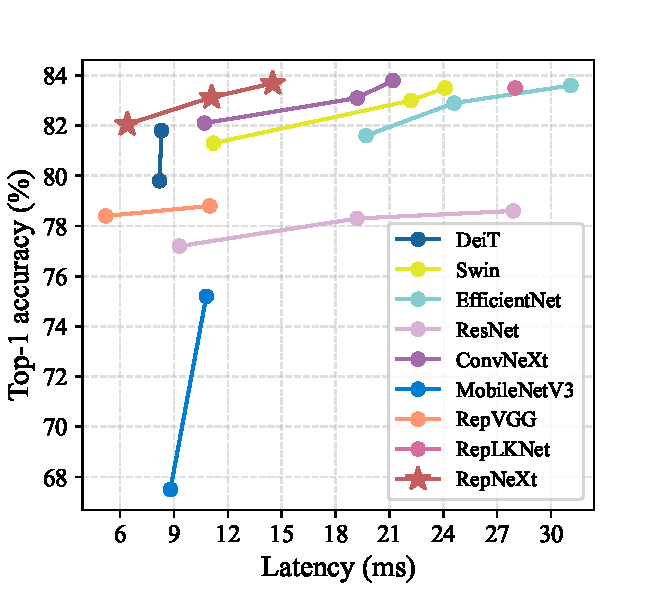
\includegraphics[width=0.7\textwidth]{figs/fig1.pdf}
  \caption{Top-1 accuracy on ImageNet-1K vs. latency. The latency is tested on an NVIDIA A100 GPU with an input resolution of $224^2$, a batch size of 1, and full precision (fp32). Spots on one line mean different versions of a model. \textbf{RepNeXt} finds a better accuracy-speed trade-off.}
  \label{fig:top}
\end{figure}

\begin{figure*}[t]
  \centering
  \begin{minipage}{0.27\linewidth}
    \centering
    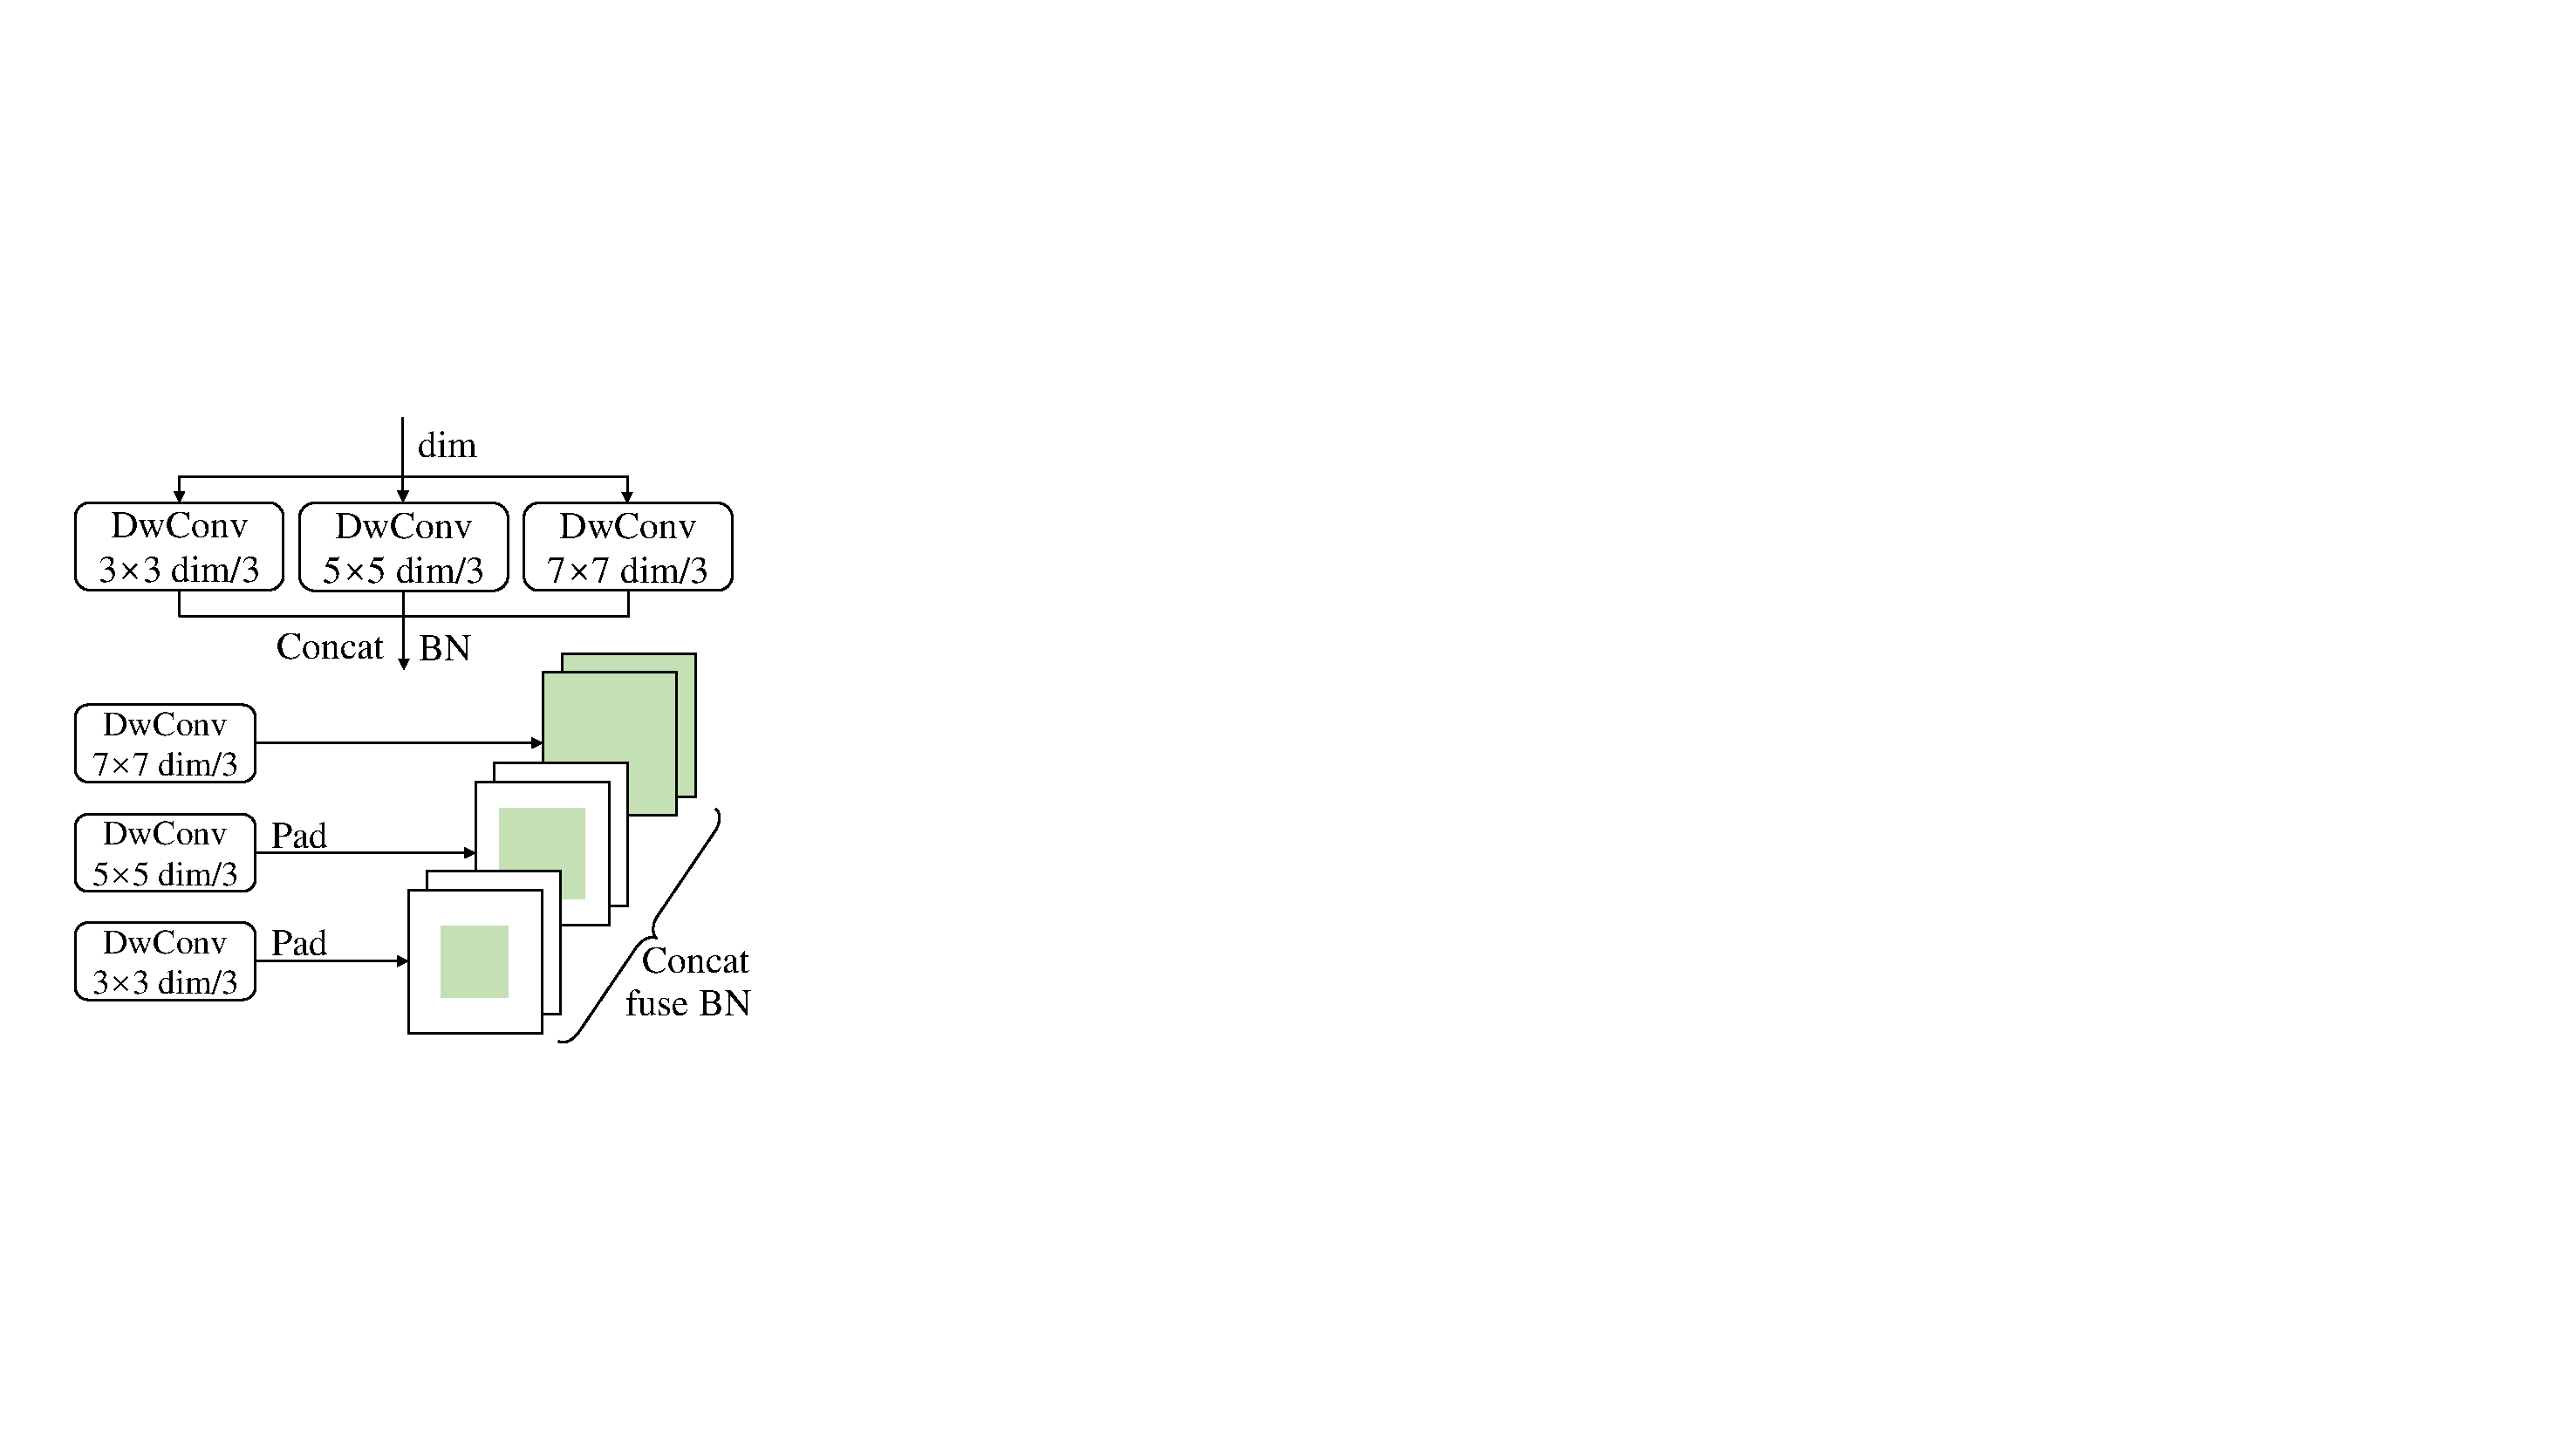
\includegraphics[height=3.6cm]{figs/fig2-a.pdf}
    \par
    (a)
    \label{fig:repunit1}
  \end{minipage}
  \hfill
  \begin{minipage}{0.34\linewidth}
    \centering
    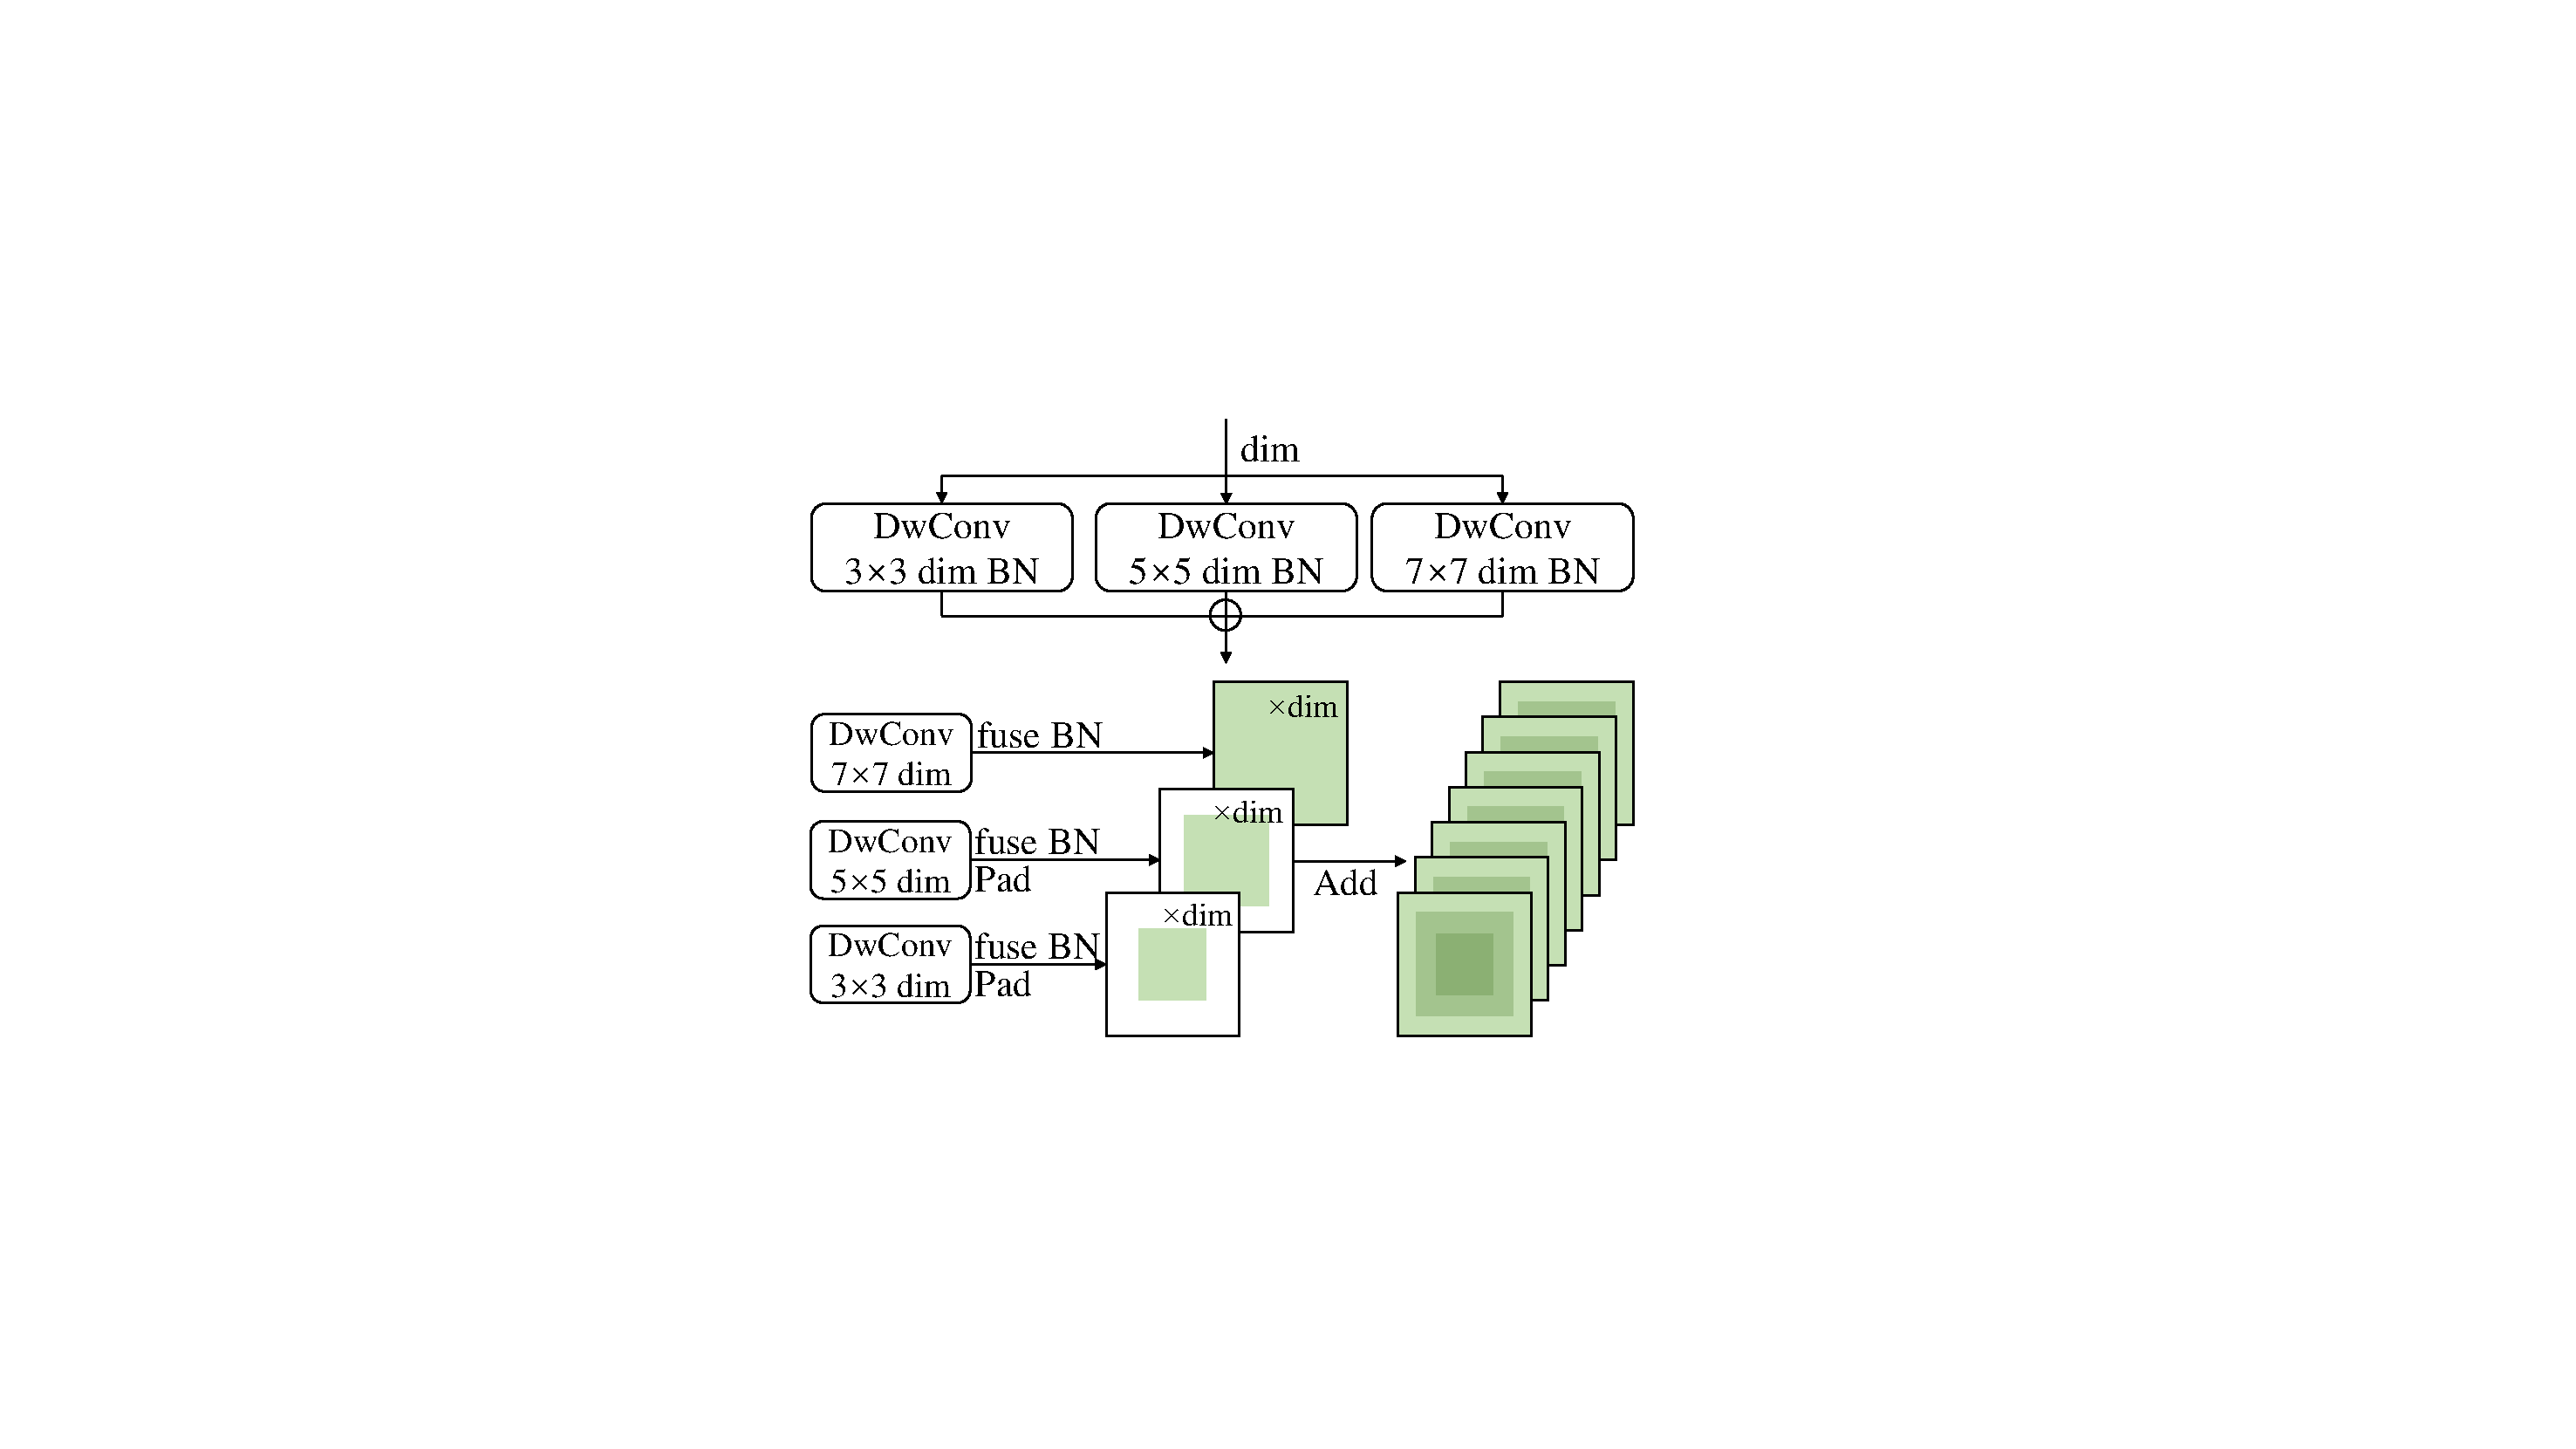
\includegraphics[height=3.6cm]{figs/fig2-b.pdf}
    \par
    (b)
    \label{fig:repunit2}
  \end{minipage}
  \hfill
  \begin{minipage}{0.34\linewidth}
    \centering
    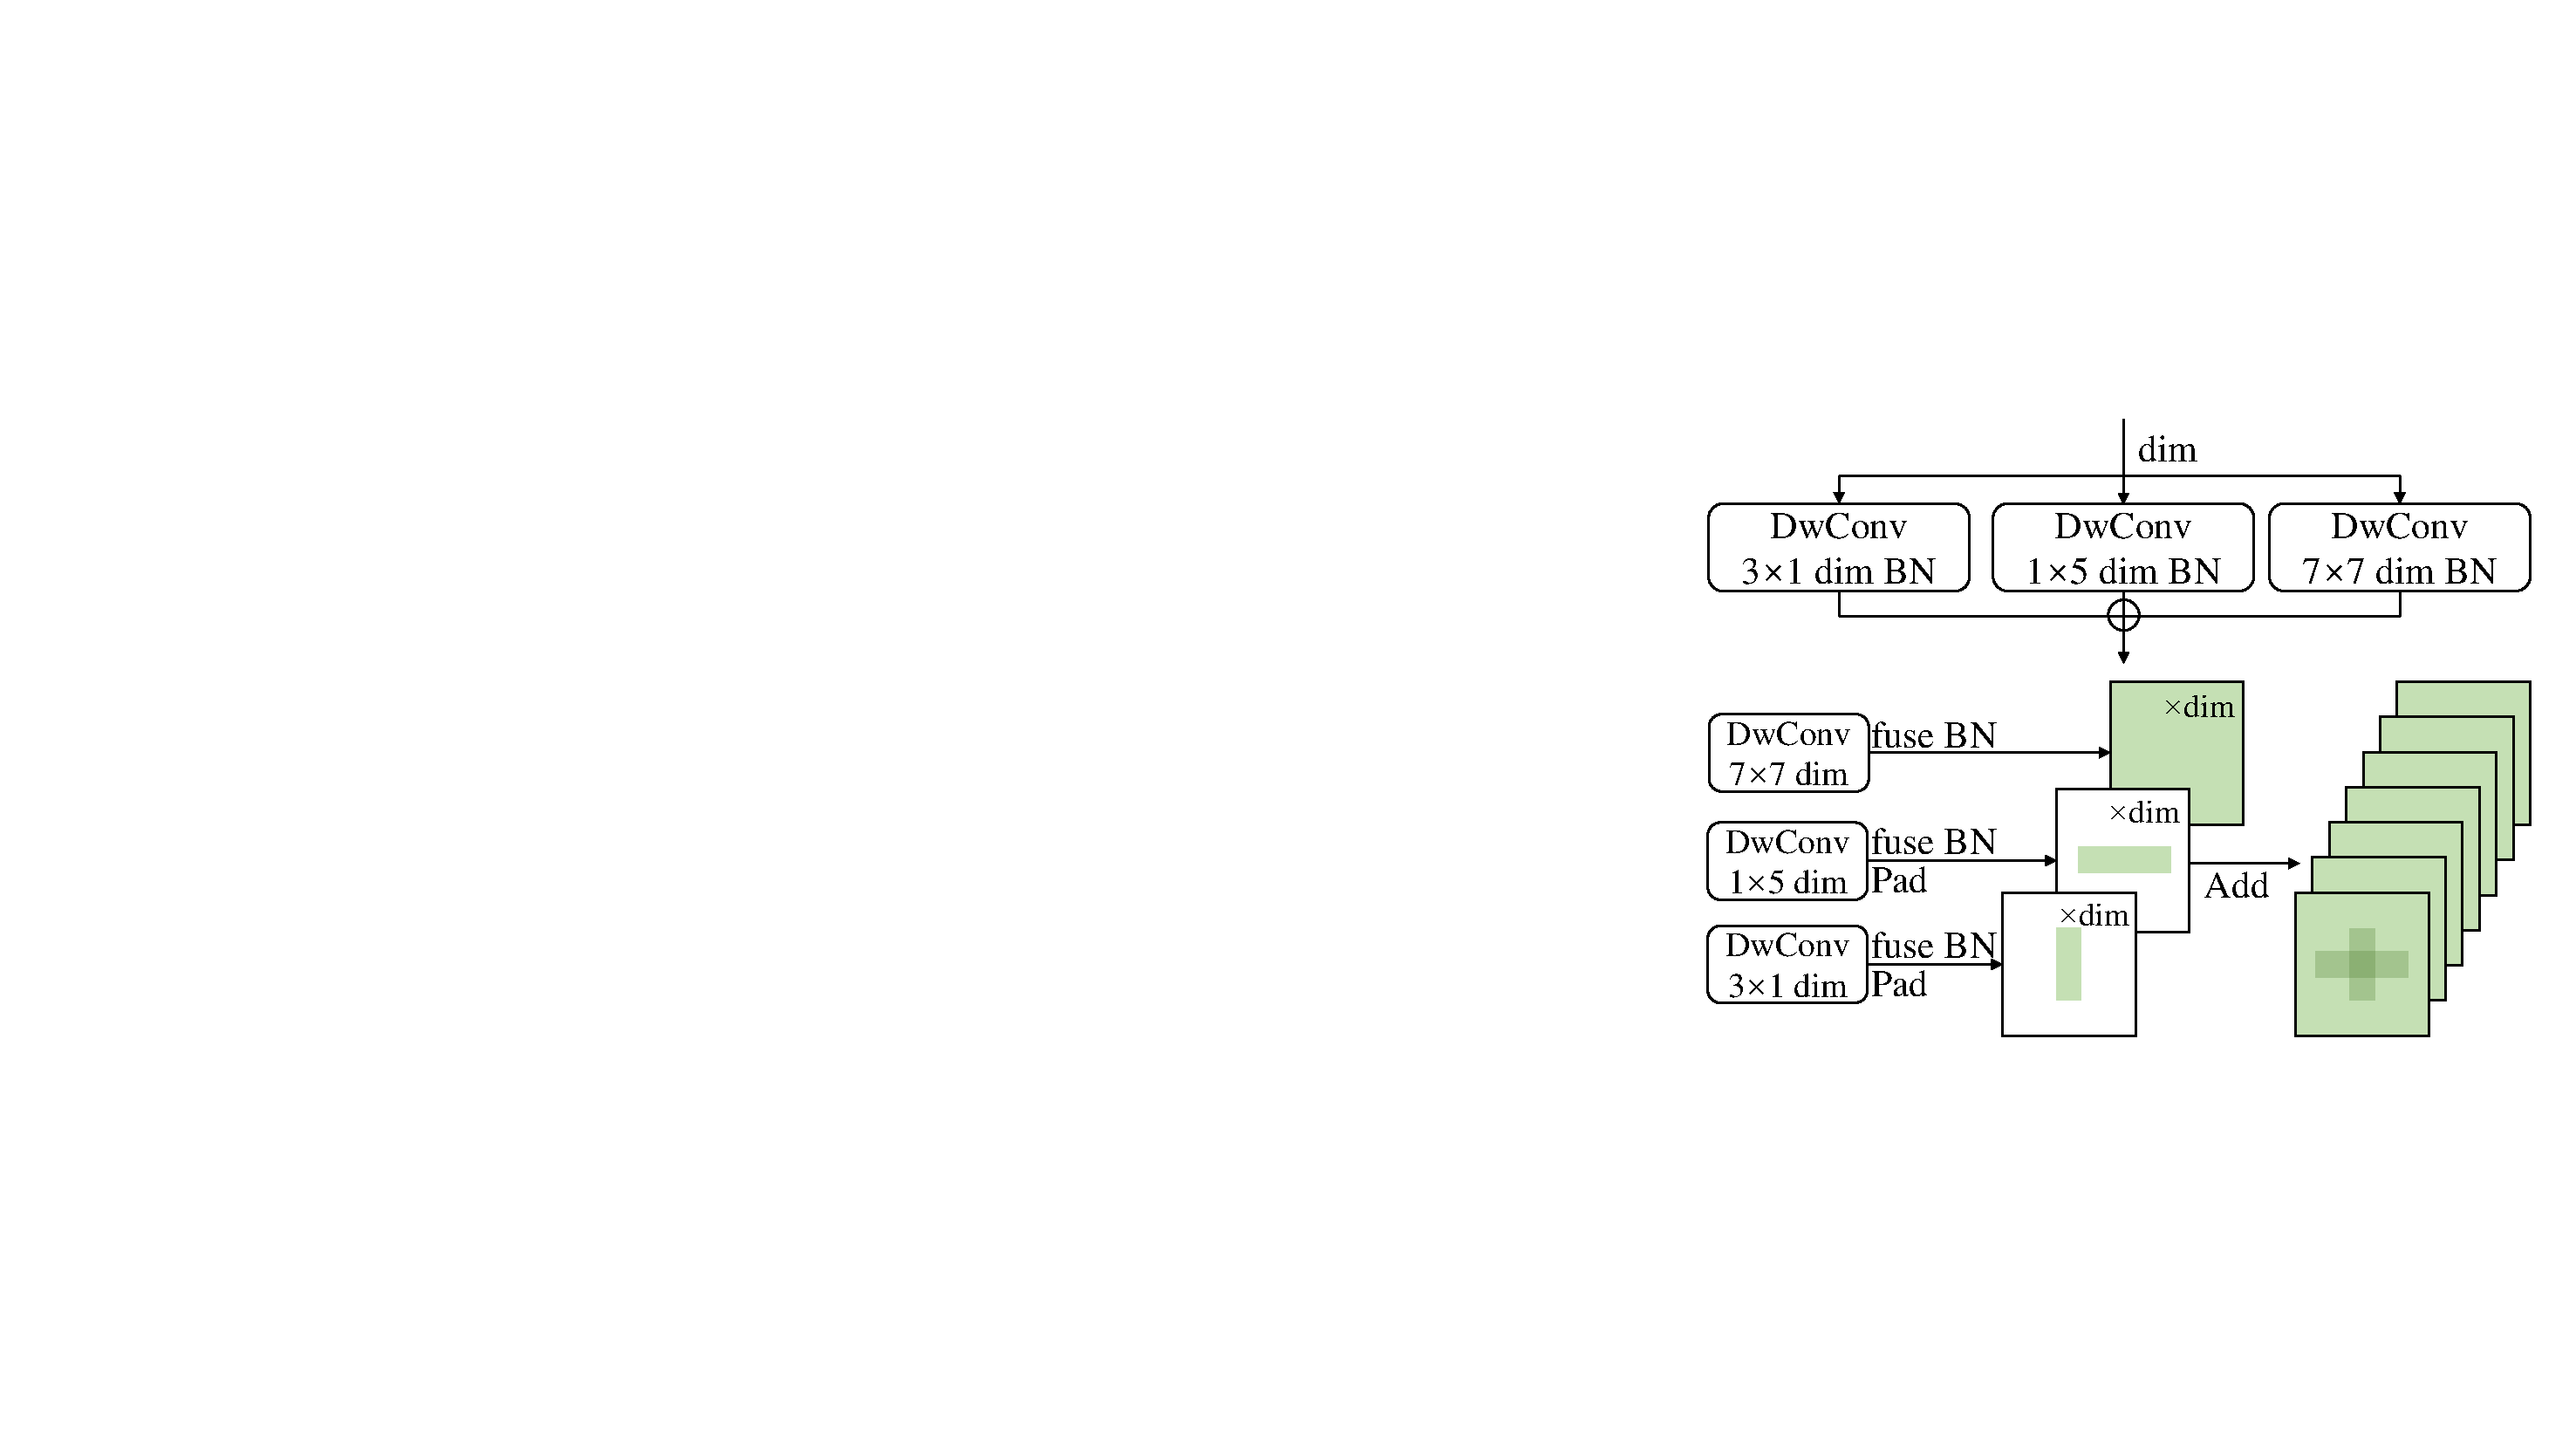
\includegraphics[height=3.6cm]{figs/fig2-c.pdf}
    \par
    (c)
    \label{fig:repunit3}
  \end{minipage}
  \caption{The \textbf{design route} and \textbf{re-parameterization process} for RepUnit. \textbf{RepUnit1 (a)} is implemented using three different sizes of parallel kernels for depth concatenation. This design style sacrifices a portion of the large receptive field to the small receptive field. Unlike RepUnit1, the implementation of \textbf{RepUnit2 (b)} uses parallel kernels for branch addition. This design style adds the small receptive field. \textbf{RepUnit3 (c)} is obtained by compressing some of the kernels of RepUnit2.}
  \label{fig:repunits}
\end{figure*}

Structural re-parameterization \cite{dbb} decouples a model into a training-time structure and an inference-time structure, which are linearly equivalent in the inference time. The training-time structure is generally designed to be complex to obtain higher performance. After training, the model is re-parameterized into a relatively simple inference-time structure to avoid increasing its inference burden. Although structural re-parameterization is often used to improve the performance of networks, its potential for inference acceleration needs to be further explored, expanded and practiced. 

We consider implementing a ConvNet that combines high performance and efficiency by fully exploiting the potential of structural re-parameterization. RepNeXt is thus proposed. \textbf{To guarantee high performance}, A re-parameterizable structure RepUnit is designed as the main feature extractor, which consists of conv layers of different scales in parallel, closer to the concept of dynamic receptive field \cite{vit} and more capable of extracting texture bias. \textbf{To guarantee good efficiency}, RepUnit is re-parameterized into a single conv layer in the inference time to reduce the inference burden. Efficient and re-parameterization-friendly components, such as BN and pointwise conv layers implemented by conv layers, are used to frame our network. Shortcut branches in the network are eliminated in an innovative and generalized way to improve memory access and parallelism. In general, RepNeXt is a re-parameterizable network. \textbf{In the training time}, shortcut branches and multi-branch feature extraction structures are present to obtain higher performance and achieve adaptation to low-resolution and fine-grained tasks. \textbf{In the inference time}, branching structures are re-parameterized into plain structures to improve inference efficiency. 
As shown in Fig. \ref{fig:top}, RepNeXt surpasses most popular lightweight and re-parameterizable networks, and obtains the same level of performance as EfficientNet and ConvNeXt on ImageNet-1K \cite{imagenet}. RepNeXt's inference is noticeably faster than most SOTA models in a variety of practical application devices.

\section{Related Work}
\label{sec:relatedwork}

\subsection{ConvNet's high-performance design paradigm}
\label{subsec:2-1}
 
\textbf{Combining the advantages of ConvNets and ViTs} is a high-performance model design trend. CoAtNet \cite{coatnet} replaced the shallow layers of a ViT with conv layers to extract universal features, incorporated certain translation invariance in the transformer structure of little prior knowledge, and showed excellent performance. BoTNet \cite{botnet} used multi-head self-attention (MHSA) to replace the $3 \times 3$ conv layers in ResNet \cite{resnet}, which greatly improved its performance. \textbf{Mimicking the structure of ViTs} to design ConvNets can also achieve good performance. Inspired by ViTs' large receptive fields, RepLKNet \cite{replknet} explored the use of very large kernels to enable ConvNets to outperform ViTs. To avoid the difficulty of extracting texture bias of large kernels, small kernels were trained in parallel with them, and the two were merged in the inference time using structural re-parameterization. ConvNeXt \cite{convnext} achieved performance beyond Swin Transformer by adopting more design ideas from ViTs. High-performance ConvNet design paradigms are rethought and summarized as follows: the use of vit-style stem, larger kernel, layer normalization, depthwise conv, pointwise conv, wider layer, inverted bottleneck structure, and shortcut branch.

\subsection{Structural Re-parameterization}
\label{subsec:2-2}

There are \textbf{6 rudimentary paradigms for ConvNet's structural re-parameterization}. \textbf{1)} A conv layer and its subsequent BN layer can be merged into a single conv layer. \textbf{2)} Multiple parallel conv layers for branch addition can be merged into a single conv layer by element-wise adding their parameters. \textbf{3)} Multiple parallel conv layers for depth concatenation can be merged into a single conv layer by concatenating their parameters. \textbf{4)} The way for merging parallel conv layers of different sizes is the same as paradigms 2 and 3 in principle, but the only difference is that all kernels need to be padded with zero to the same size as the largest one. \textbf{5)} A pointwise conv layer and a conv layer in series can be merged into a single conv layer leveraging the associative axiom of convolutional operations.  \textbf{6)} A pooling or BN layer can be converted into a conv layer to facilitate other structural re-parameterization operations.

\textbf{Structural re-parameterization} has recently received much attention as a way to improve performance by decoupling a model into its training-time structure and inference-time structure. ACNet \cite{acnet} and DBB \cite{dbb} respectively used two re-parameterizable structures of different complexity to replace the $K \times K$ conv in the original network, which greatly improved the performance. RepVGG \cite{repvgg} used a re-parameterizable structure containing a shortcut branch with a BN layer, allowing the model to be trained with multiple branches and to infer like with one branch. \cite{rmnet} has preliminarily demonstrated that Dirac initialization can be employed to equivalently represent shortcut branches. As more recent research works, RepGhost \cite{repghost}, ResRep \cite{resrep}, and RepMLP \cite{repmlp} utilized Rep to explore the effects of a better accuracy-speed trade-off, Rep-guided network pruning, and joint feature extraction by fully-connected layers (for long-range modeling) and conv layers (for local modeling), respectively.

The proposed RepNeXt, in contrast to existing re-parameterization methods, neither employs a redundant feature extraction structure like DBB nor a re-parameterization trick that simulates shortcut branches (shortcut branches correspond to only one layer of main branches and are not suitable for building deep networks) like RepVGG. The simple and multi-scale feature extraction structure and realistic shortcut branch re-parameterization will contribute to the high performance and efficiency of RepNeXt.

\section{RepNeXt}
\label{sec:repnext}

\subsection{Re-parameterizable Block Design}
\label{sec:3-1}

Using larger kernels proved beneficial for the ImageNet classification task \cite{replknet}. However, experiments (cf., Tables \ref{table:imagewoof} and \ref{table:cifar100}) show that using purely large kernels is difficult to achieve satisfactory results as on ImageNet on fine-grained and low-resolution tasks. This phenomenon is because the texture bias is more critical \textbf{for fine-grained tasks}, yet large kernels are more concerned with extracting the shape bias. \textbf{For low-resolution tasks}, the texture bias is inherently insufficient, and ignoring it degrades the recognition performance.

We consider using structural re-parameterization to extract both texture and shape bias in the training time without increasing the inference burden. Concretely, we design a re-parameterizable structure called RepUnit for feature extraction, whose inference-time structure is a depthwise conv layer of size $7 \times 7$. With the design principle of not increasing the training cost excessively and the coexistence of large and small kernels, the design route and re-parameterization process for RepUnit are shown in Fig. \ref{fig:repunits}.

RepUnit1 (cf., Fig. \ref{fig:repunits}(a)) uses three parallel depthwise conv layers of different sizes for feature extraction in the training time. The depthwise conv layer of each size receives one-third of the input feature map, and the outputs of all layers are concatenated as the output feature map. To describe the re-parameterization process, the three depthwise conv kernels are defined as $F_1 \in \mathbb{R}^{\frac{dim}{3} \times 1 \times 3 \times 3}$, $F_2 \in \mathbb{R}^{\frac{dim}{3} \times 1 \times 5 \times 5}$ and $F_3 \in \mathbb{R}^{\frac{dim}{3} \times 1 \times 7 \times 7}$. The input feature map is defined as $I \in \mathbb{R}^{dim \times H \times W}$. The output feature map is defined as $O \in \mathbb{R}^{dim \times H \times W}$. The running mean, running var, weight, and bias of the BN Layer are defined as $\mu$, $\sigma$, $\gamma$, and $\beta$. In the training time, the forward propagation of RepUnit1 can be described as \eqref{eq1}.

\begin{equation}
\begin{aligned}
    O=({\rm cat}(F_1 * I[0:\frac{dim}{3}], F_2 * I[\frac{dim}{3}:\frac{2 \cdot dim}{3}],\\ F_2 * I[\frac{2 \cdot dim}{3}:]) - \mu) \frac{\gamma}{\sigma}+\beta,
    \label{eq1}
\end{aligned}
\end{equation}

\noindent
where ${\rm cat}$ means concatenation, $*$ means the convolutional operation, and $[:]$ means the slice operation. According to the associative axiom of the convolutional operation, \eqref{eq2} is equivalent to \eqref{eq1}.

\begin{equation}
   O = \frac{\gamma}{\sigma}{\rm cat}({\rm pad}(F_1), {\rm pad}(F_2), F_3)*I -\frac{\gamma\mu}{\sigma} + \beta,
    \label{eq2}
\end{equation}

\noindent
where ${\rm pad}$ means padding a kernel with zeros to $7 \times 7$ size. RepUnit1 can be re-parameterized into a single conv layer, whose forward propagation can be described as $O = \hat{F}*I + \hat{B}$, where $\hat{F}=\frac{\gamma}{\sigma}{\rm cat}({\rm pad}(F_1), {\rm pad}(F_2), F_3)$ and $\hat{B} =-\frac{\gamma\mu}{\sigma} + \beta$. The design of RepUnit1 is attractive because the presence of smaller kernels and the non-increased layer width decrease the training cost.

Since there is no guarantee that every channel of the input feature map can be fed into the most appropriate branch, we design RepUnit2 (cf., Fig. \ref{fig:repunits}(b)). Each branch accepts the complete input feature map. The final output feature map results from the element-wise addition of the output feature map through each branch after batch normalization. The scaling function of the normalization layer is essential for multi-branch structures, which plays a role in controlling the saliency of branches \cite{online}. Let $F_1 \in \mathbb{R}^{dim \times 1 \times 3 \times 3}$, $F_2 \in \mathbb{R}^{dim \times 1 \times 5 \times 5}$, and $F_3 \in \mathbb{R}^{dim \times 1 \times 7 \times 7}$ be the three parallel depthwise conv kernels. Let $\mu_i$, $\sigma_i$, $\gamma_i$, and $\beta_i$ be the parameters of the $i$th BN layer, the forward propagation of RepUnit2 in the training time can be described as \eqref{eq3}.

\begin{figure}
  \centering
  \begin{minipage}{0.49\linewidth}
    \centering
    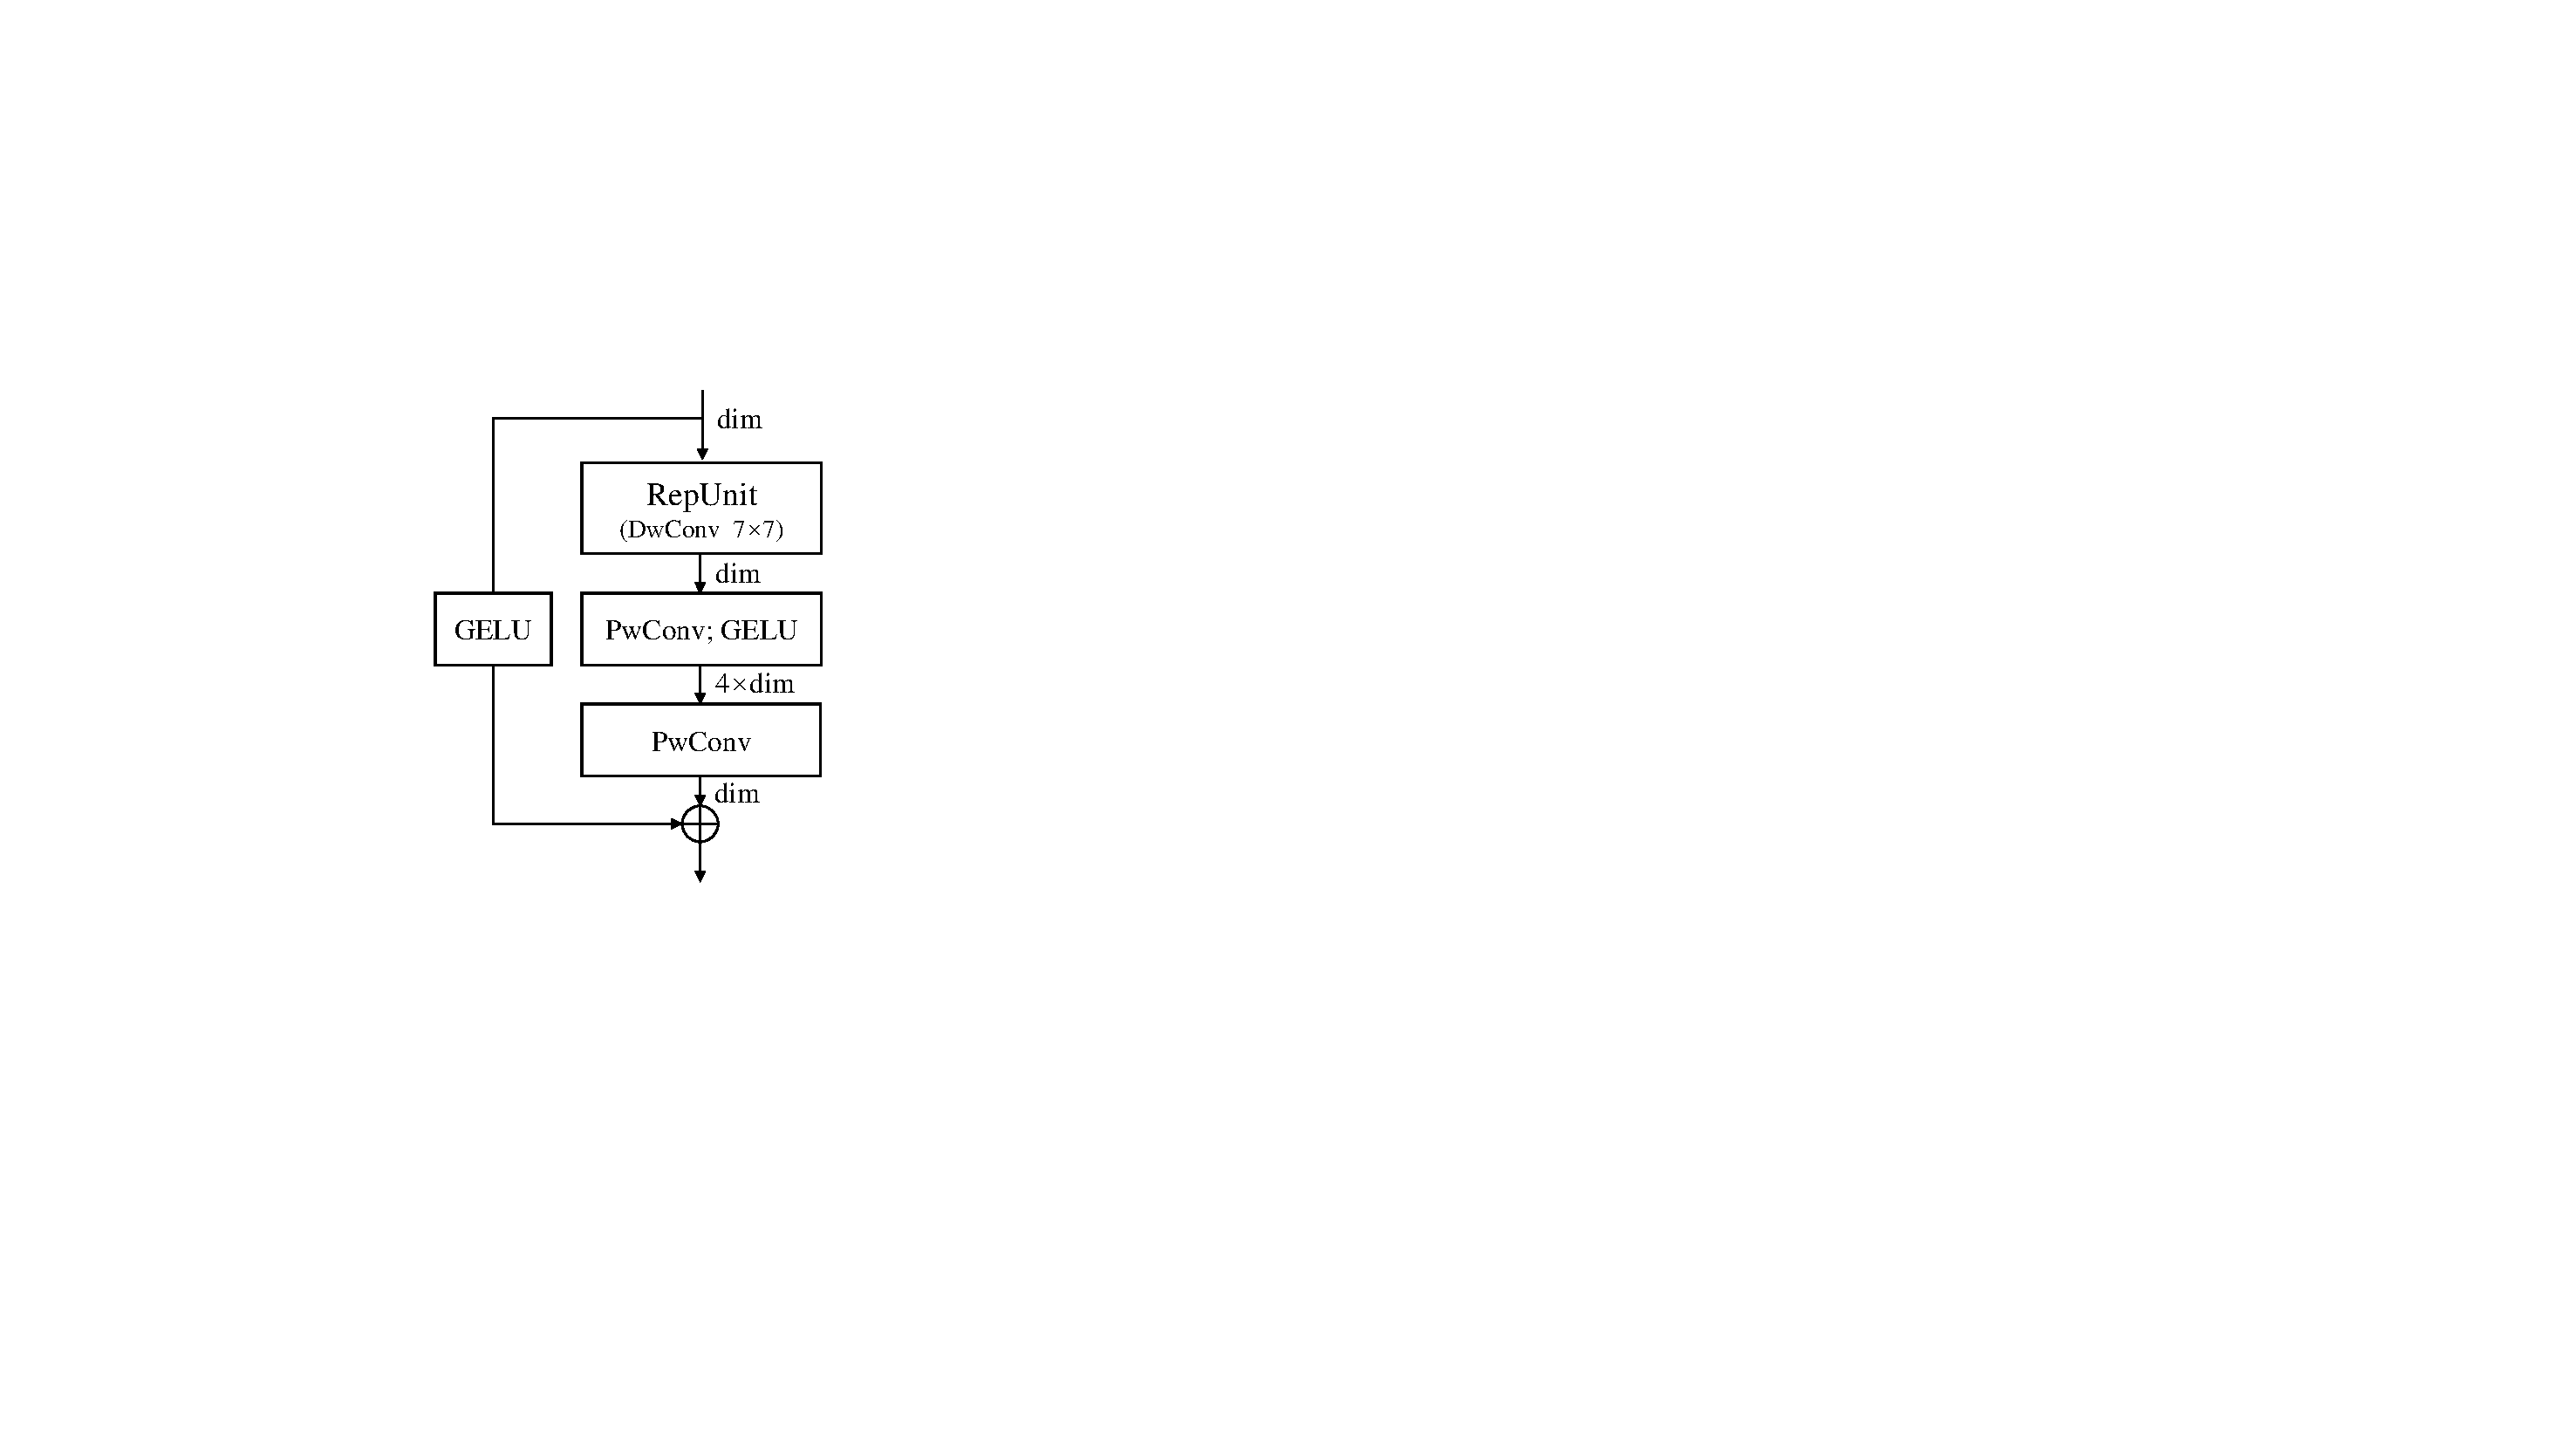
\includegraphics[height=5.6cm]{figs/fig3-a.pdf}
    \par
    (a)
    \label{fig:repnext-train}
  \end{minipage}
  \hfill
  \begin{minipage}{0.49\linewidth}
    \centering
    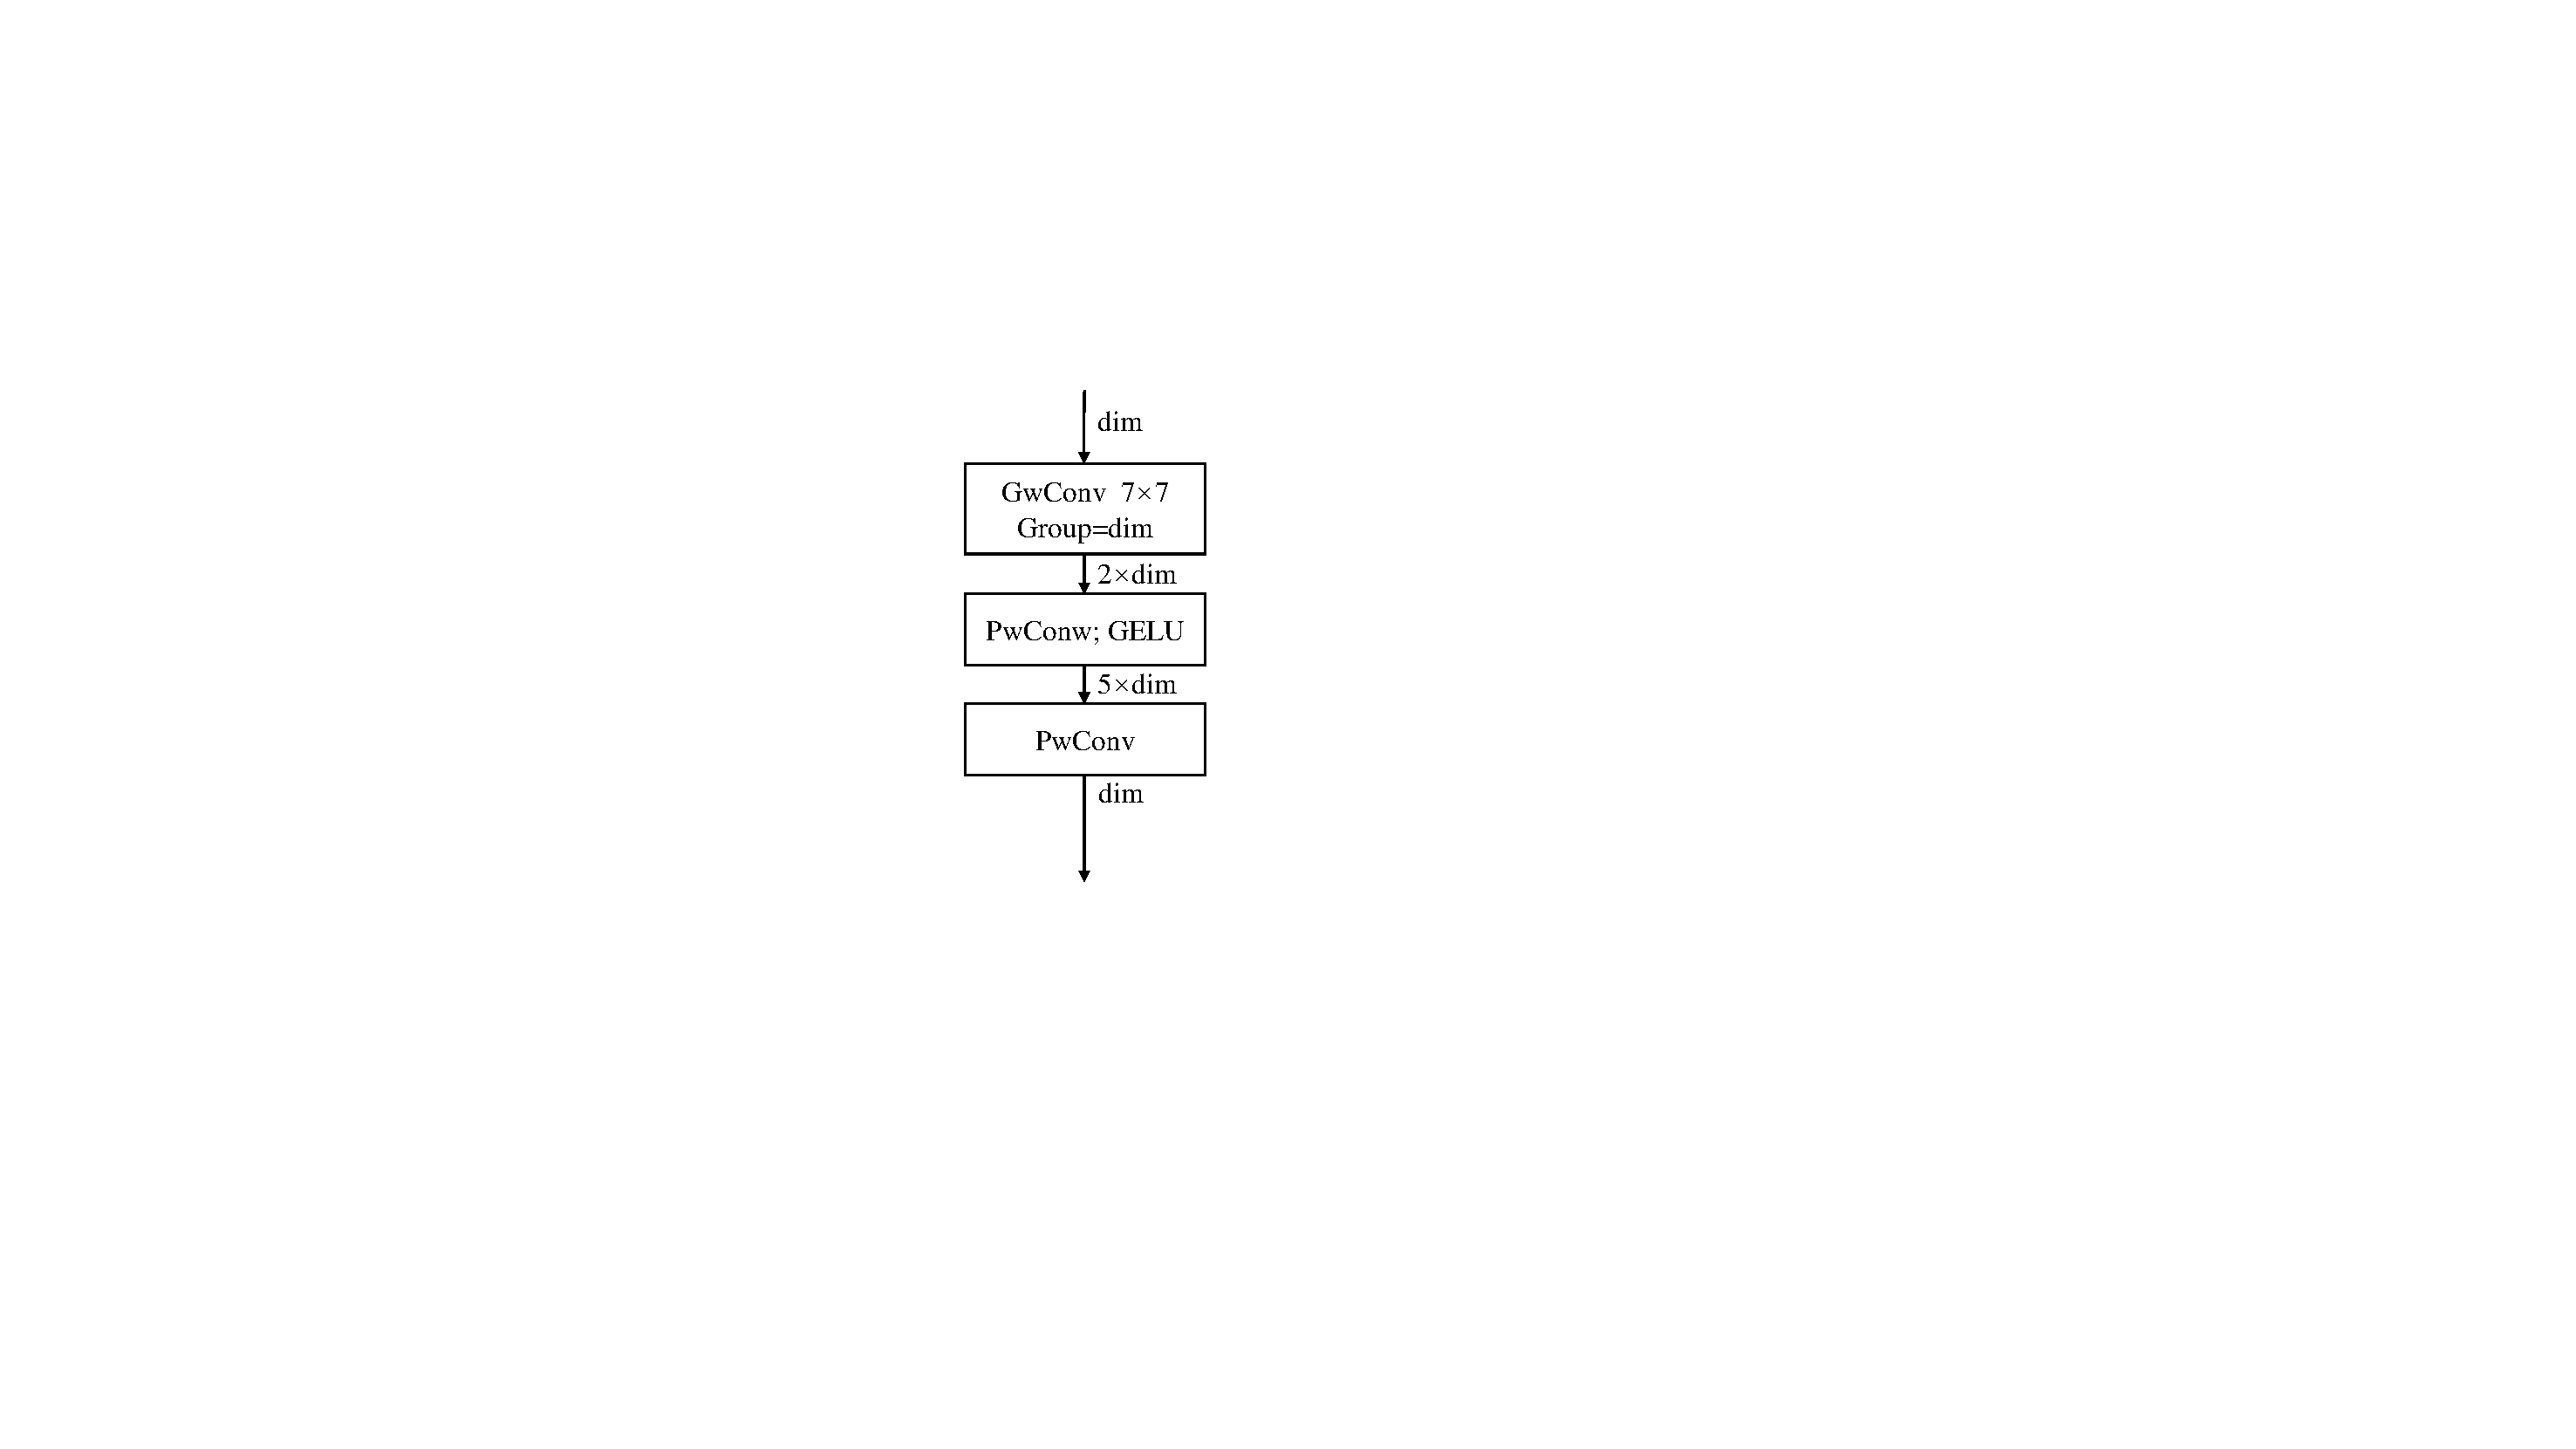
\includegraphics[height=5.6cm]{figs/fig3-b.pdf}
    \par
    (b)
    \label{fig:repnext-infer}
  \end{minipage}
  \caption{\textbf{Block designs} for a training-time RepNeXt \textbf{(a)}, and an inference-time RepNeXt \textbf{(b)}. RepNeXt uses RepUnit as the main feature extractor, uses the BN layer for normalization, uses pointwise conv to implement inverted bottlenecks, and adds an activation layer to the shortcut branch. After re-parameterization, RepNeXt will become a branchless plain architecture.}
  \label{fig:blocks}
\end{figure}

\begin{figure*}
  \centering
  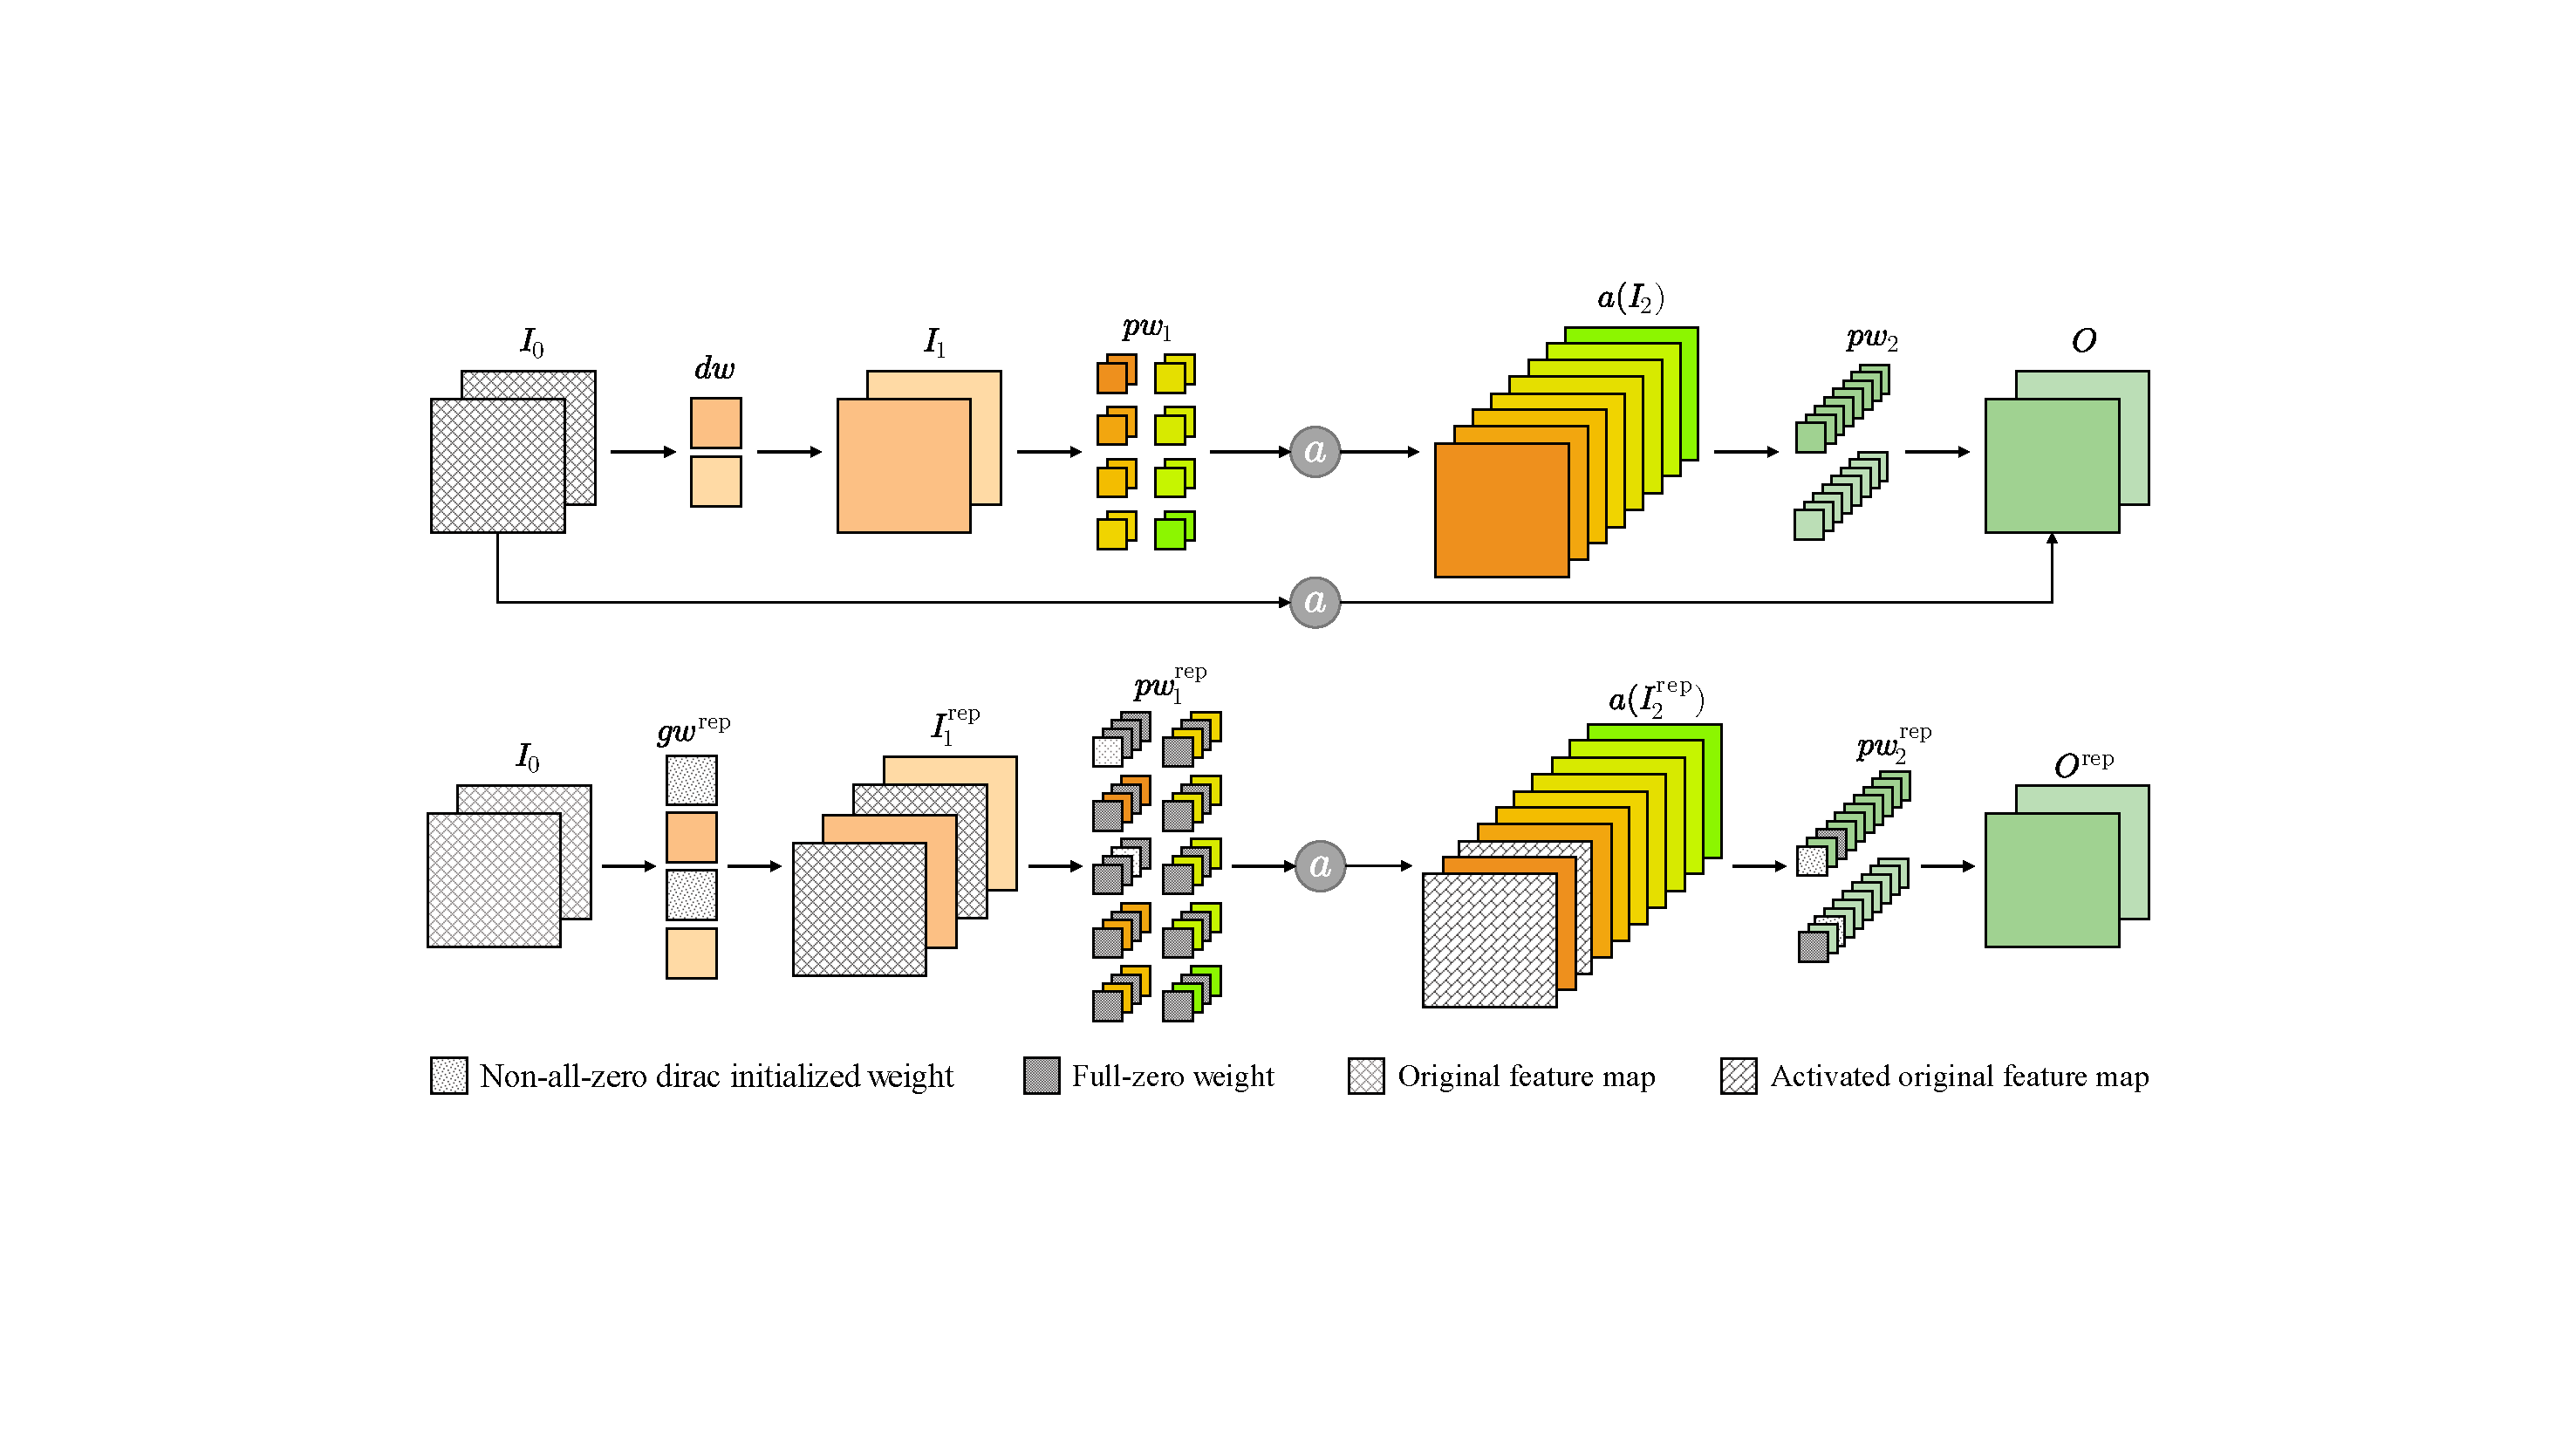
\includegraphics[width=\textwidth]{figs/fig4.pdf}
  \caption{\textbf{Shortcut re-parameterization} for RepNeXt. The upper and lower parts represent the RepNeXt block before and after the shortcut re-parameterization. Equivalent elimination of the shortcut branch is achieved by dirac initialization as the core tool with the prerequisite that the shortcut branch contains the same activation layer as the main branch.}
  \label{fig:shortcutrep}
\end{figure*}

\begin{equation}
   O=\sum_{i=1}^3 ((F_i * I-\mu_i) \frac{\gamma_i}{\sigma_i}+\beta_i).
    \label{eq3}
\end{equation}

Equation \eqref{eq4} is equivalent to \eqref{eq3} according to the associative axiom of the convolutional operation.

\begin{equation}
   O = (\sum_{i=1}^2{\rm pad}(\frac{\gamma_iF_i}{\sigma_i}) +\frac{\gamma_3F_3}{\sigma_3}) * I + \sum_{i=1}^3(\beta_i - \frac{\mu_i\gamma_i}{\sigma_i}).
    \label{eq4}
\end{equation}

Thus RepUnit2 can be re-parameterized as a single conv layer, whose forward propagation can be described as $O = \hat{F}*I + \hat{B}$, where $\hat{F}=\sum_{i=1}^2{\rm pad}(\frac{\gamma_iF_i}{\sigma_i}) +\frac{\gamma_3F_3}{\sigma_3}$ and $\hat{B} =\sum_{i=1}^3(\beta_i - \frac{\mu_i\gamma_i}{\sigma_i})$. RepUnit2 has more parameters and a larger width, which will increase the training cost, although it does not affect the inference speed.

To reduce the training cost, we design RepUnit3 (cf., Fig. \ref{fig:repunits}(c)), which compresses the depthwise conv kernel of size $3 \times 3$ to $3 \times 1$ and the depthwise conv kernel of size $5 \times 5$ to $1 \times 5$ based on RepUnit2, whose re-parameterization procedure is the same as RepUnit2.

When designing the RepNeXt block, we take adequate advantage of the high-performance design paradigm previously mentioned to maintain good performance. 
But when efficiency is considered, the LN layer is not suitable for subsequent acceleration operations such as operator fusion because it distinguishes between individual samples rather than individual channels for normalization. In addition, using a fully connected layer to implement pointwise conv relies on frequent dimensional transformations, which is an efficiency-unfriendly fragmentation operation, even though pointwise conv and fully connected layers can be transformed into each other. Therefore, we use BN and pointwise conv layers implemented by conv layers to form the RepNeXt block. Furthermore, an activation layer is added to the shortcut branch to facilitate the re-parameterization for shortcut branches (cf., Section \ref{sec:3-2}). The training-time RepNeXt block (cf., Fig. \ref{fig:blocks}(a)) is thus formed. After training, the network is re-parameterized to obtain the inference-time RepNeXt, whose block is shown in Fig. \ref{fig:blocks}(b).


\subsection{Shortcut Re-parameterization}
\label{sec:3-2}

The number of parameters and the floating-point operations (FLOPs) may no longer describe modern multi-branch models' efficiency as reasonably and straightforwardly as the inference latency. Multiple branches increase the memory footprint \cite{repvgg}. A high memory footprint implies a low degree of parallelism \cite{mobilenetv3}, which slows down the model's inference and is an obstacle to applying the model to real-time inference scenarios. Hence, shortcut re-parameterization is valuable. 

\cite{rmnet} proves that dirac initialization can eliminate shortcut branches in a network. However, it depends on the non-negativity of ReLU. We have innovatively eliminated this dependency and provided solutions for shortcut re-parameterization in the presence of more layers in the main branch, groupwise conv, and inconsistent input and output channels. Fig. \ref{fig:shortcutrep} illustrates the shortcut re-parameterization process of the RepNeXt block. The core tool for shortcut re-parameterization is dirac initialization, which aims to make the input and output feature map identical. The dirac initialization of a kernel $K \in \mathbb{R}^{O \times I \times H \times W}$ can be described as \eqref{eq5}.

\begin{equation}
\begin{aligned}
    K_{o,i,h,w} = \begin{cases}1& {\rm if} \ \ h=\frac{H}{2}, w=\frac{W}{2}, o=i,\\0& {\rm elsewise}.\end{cases}
    \label{eq5}
\end{aligned}
\end{equation}

The output dimension of all conv layers except the last one is increased, and the corresponding weights are dirac initialized. Thus, the original feature map can appear in the output feature map in a \textbf{concatenated} form. The input dimension of the last conv layer is increased, and the corresponding weights are also dirac initialized. Thus, the element-wise addition of the original feature map and the output feature map of the main branch can be equivalently converted into a \textbf{convolutional operation}. Some concrete instructions are as follows: \textbf{1)} Dirac-initialized kernels need to be inserted into the depthwise conv layer one after another to form a groupwise conv layer (group$=$dim) because adjacent kernels are always used as a group. \textbf{2)} To accommodate instruction 1, dirac-initialized kernels must also be inserted into the first pointwise conv layer one after another. Some additional all-zero weights need to be introduced in the input dimension, as $pw_1^{\rm rep}$ in Fig. \ref{fig:shortcutrep} demonstrates. \textbf{3)} To adapt shortcut re-parameterization to various activation layers, instead of relying on the prerequisite that the feature map remains non-negative after ReLU \cite{rmnet}, we add an activation layer on the shortcut branch that is identical to the main branch. 

In this way, a re-parameterized plain architecture can be obtained to replace the training-time architecture and does not change the inference results. The shortcut re-parameterization converts the extra memory footprint and the element-wise addition operation into a convolutional operation. In modern devices like GPUs, the element-wise addition is generally performed on Vector Units. The convolution is generally performed on Matrix Units, which has more optimizations than the former and is more efficient. This conversion improves memory access and the degree of parallelism. In addition, shortcut re-parameterization relies on hardware sparse optimization and may sacrifices some throughput for latency optimization (skipping sparse computation requires checking sparsity). Thus shortcut re-parameterization becomes an optional choice.

$O$ and $O^{\rm rep}$ are satisfying computational equivalence and can be proved as follows: 

According to Fig. \ref{fig:shortcutrep}, it is straightforward to define the kernels associated with structural re-parameterization as $gw^{\rm rep} = [dw^{{\rm C} \times 1}, E^{{\rm C} \times 1}]^{2{\rm C} \times 1}, B(gw^{\rm rep}) = [B^{{\rm C}}(dw)$, $0^{{\rm C}}]^{2{\rm C}}$, 
$pw_1^{\rm rep} = [[pw_1^{4{\rm C} \times {\rm C}}, 0^{{\rm C} \times {\rm C}}]^{5{\rm C} \times {\rm C}}, [0^{4{\rm C} \times {\rm C}}$, $E^{{\rm C} \times {\rm C}}]^{5{\rm C} \times {\rm C}}]^{5{\rm C} \times 2{\rm C}}$, 
$B(pw_1^{\rm rep}) = [B^{4{\rm C}}(pw_1), 0^{{\rm C}}]^{5{\rm C}}$,
$pw_2^{\rm rep}=[pw_2^{{\rm C} \times 4{\rm C}}$, $E^{{\rm C} \times {\rm C}}]^{{\rm C} \times 5{\rm C}}, B(pw_2^{\rm rep})=B^{\rm C}(pw_2)$, where $[\cdot, \cdot]$ means the depth concatenation of the two or more elements, and $E$ means the dirac initialized weights. For ease of understanding, the dimensions of noticeable elements have been marked in their upper right.

\begin{table*}[t]
\centering
\small
\begin{adjustbox}{center}
\begin{tabular}{cc|c|c}
\multicolumn{1}{c|}{Structure} & Output Size & Training-time RepNeXt & Inference-time RepNeXt \\ \hline
\multicolumn{1}{c|}{Stem} & 56 $\times$ 56 & $\begin{array}{c} 4 \times 4,s=4,96 \\ BN \end{array}$ & $4 \times 4,s=4,96$ \\ \hline
\multicolumn{1}{c|}{Stage1} & 56 $\times$ 56 & $\bigg [\begin{array}{c}\text { RepUnit, } d w, 96 \\ 1 \times 1,384 \\ 1 \times 1,96\end{array}\bigg ] \times 3$ & $\bigg [\begin{array}{c}7 \times 7,192, \text { group }=96 \\ 1 \times 1,480 \\ 1 \times 1,96\end{array}\bigg ] \times 3$ \\ \hline
\multicolumn{1}{c|}{Stage2} & 28 $\times$ 28 & $\bigg [\begin{array}{c}\text { RepUnit, } d w, 192 \\ 1 \times 1,768 \\ 1 \times 1,192\end{array}\bigg ] \times 3$ & $\bigg [\begin{array}{c}7 \times 7,384, \text { group }=192 \\ 1 \times 1,960 \\ 1 \times 1,192\end{array}\bigg ] \times 3$ \\ \hline
\multicolumn{1}{c|}{Stage3} & 14 $\times$ 14 & $\bigg [\begin{array}{c}\text { RepUnit, } d w, 384 \\ 1 \times 1,1536 \\ 1 \times 1,384\end{array}\bigg ] \times 9$ & $\bigg [\begin{array}{c}7 \times 7,768, \text { group }=384 \\ 1 \times 1,1920 \\ 1 \times 1,384\end{array}\bigg] \times 9$ \\ \hline
\multicolumn{1}{c|}{Stage4} & 7 $\times$ 7 & $\bigg [\begin{array}{c}\text { RepUnit, } d w, 768 \\ 1 \times 1,3072 \\ 1 \times 1,768\end{array}\bigg ] \times 3$ & $\bigg [\begin{array}{c}7 \times 7,1536, \text { group }=768 \\ 1 \times 1,3840 \\ 1 \times 1,768\end{array}\bigg ] \times 3$ \\ %\hline
% \multicolumn{2}{c|}{FLOPs} & 4.5B & 8.2B \\ \hline
% \multicolumn{2}{c|}{\#Params.} & 29M & 52M \\ \hline
% \multicolumn{2}{c|}{speed} & 11.9  &  6.6  \\ 
\end{tabular}
\end{adjustbox}
\caption{\textbf{Detailed architecture specification} for the training-time RepNeXt-T and the inference-time RepNeXt-T. The resolution of the image input to the models is $224^2$.}
\label{table:architecture}
\end{table*}

Let us calculate the intermediate results in the order of forward propagation. $I_1^{\rm rep}$ can be derived as \eqref{eq6}.

\begin{equation}
    \begin{aligned}
    I_1^{\rm rep} &= gw^{\rm rep} * I_0^{\rm C} + B(gw^{\rm rep})\\&= [dw^{{\rm C} \times 1}, E^{{\rm C} \times 1}]^{2{\rm C} \times 1} * I_0^{\rm C} + [B^{{\rm C}}(dw), 0^{{\rm C}}]^{2{\rm C}} \\&= [dw^{{\rm C} \times 1} * I_0^{\rm C}+B^C(dw), E^{{\rm C} \times 1} * I_0^{\rm C}+0^{\rm C}] \\&= [I_1^{\rm C}, I_0^{\rm C}]^{2{\rm C}}.
    \end{aligned}
    \label{eq6}
\end{equation}

Using the results of $I_1^{\rm rep}$, ${\rm a}(I_2^{\rm rep})$ can be calculated as \eqref{eq7}, where ${\rm a}$ can be any kind of activation.

\begin{equation}
\begin{aligned}
{\rm a}(I_2^{\rm rep}) &= {\rm a}(pw_1^{\rm rep} * I_1^{\rm rep} + B(pw_1^{\rm rep}))\\
&= {\rm a}( [[pw_1^{4{\rm C} \times {\rm C}}, 0^{{\rm C} \times {\rm C}}]^{5{\rm C} \times {\rm C}}, [0^{4{\rm C} \times {\rm C}}, E^{{\rm C} \times {\rm C}}]^{5{\rm C} \times {\rm C}}]^{5{\rm C} \times 2{\rm C}} * [I_1^{\rm C}, I_0^{\rm C}]^{2{\rm C}} + [B^{4{\rm C}}(pw_1), 0^{\rm C}]^{5{\rm C}} )\\ 
% &= {\rm a}\{ [pw_1^{4{\rm C} \times {\rm C}}, 0^{{\rm C} \times {\rm C}}]^{5{\rm C} \times {\rm C}} * I_1^{\rm C} + [0^{4{\rm C} \times {\rm C}}, E^{{\rm C} \times {\rm C}}]^{5{\rm C} \times {\rm C}} * I_0^{\rm C} + [B^{4{\rm C}}(pw_1), 0^{{\rm C}}]^{5{\rm C}} \}\\
&={\rm a}([pw_1^{4{\rm C} \times {\rm C}} * I_1^{\rm C} , 0^{{\rm C}}]^{5{\rm C}} + [0^{4{\rm C}}, I_0^{\rm C}]^{5{\rm C}} + [B^{4{\rm C}}(pw_1), 0^{{\rm C}}]^{5{\rm C}})\\
&={\rm a}([pw_1^{4{\rm C} \times {\rm C}} * I_1^{\rm C} + 0^{4{\rm C}} + B^{4{\rm C}}(pw_1), 0^{\rm C} + I_0^{\rm C} + 0^{\rm C}])\\
&=[{\rm a}^{4{\rm C}}(I_2), {\rm a}^{\rm C}(I_0)]^{5{\rm C}}.
\end{aligned}
\label{eq7}
\end{equation}

Finally, we use the result of ${\rm a}(I_2^{\rm rep})$ to calculate $O^{\rm rep}$, and you will find that it is equivalent to the original output $O$.

\begin{equation}
\begin{aligned}O^{\rm rep} &= pw_2^{\rm rep} * {\rm a}(I_2^{\rm rep}) + B(pw_2^{\rm rep})\\
&= [pw_2^{{\rm C} \times 4{\rm C}}, E^{{\rm C} \times {\rm C}}]^{{\rm C} \times 5{\rm C}} * [{\rm a}^{4{\rm C}}(I_2), {\rm a}^{\rm C}(I_0)]^{5{\rm C}} + B^{\rm C}(pw_2) \\ 
&= pw_2^{{\rm C} \times 4{\rm C}} * {\rm a}^{4{\rm C}}(I_2) + B^{\rm C}(pw_2) + {\rm a}^{\rm C}(I_0)\\
&= O.\end{aligned}
\label{eq8}
\end{equation}

\subsection{Architecture Specification}
\label{sec:3-3}

We define the architecture of RepNeXt in Table \ref{table:architecture}.

\textbf{Stem} denotes the previous few layers of the network. Following the concept of patch embedding, our stem consists of a conv layer of size and stride equal to 4 and a BN layer. The reason for using batch normalization instead of layer normalization is that it can be merged with the conv layer (Rep. Paradigm 1) to accelerate inference.

\textbf{stage1 to stage4} each contains several RepNeXt blocks (cf., Fig. \ref{fig:blocks}(a)). In the training time, each block contains a RepUnit for feature extraction, two pointwise conv layers for implementing the inverted bottleneck structure, and a shortcut branch with an activation layer (not shown in Table \ref{table:architecture}). After training and structural re-parameterization, each block in the stage contains a groupwise conv layer of $7 \times 7$ size, two pointwise conv layers with different input or output dimensions from the training-time block, and no more multiple branches (cf., Fig. \ref{fig:blocks}(b)).

\textbf{Downsampling layers} (not shown in Table \ref{table:architecture}) are located between stages and consist of a BN layer and a conv layer of size and stride equal to 2. Downsampling layers are responsible for downsampling the input feature map to half its size and doubling the number of output channels. The case where the BN layer is in front of the conv layer can also be re-parameterized. The BN layer is equivalently converted into a pointwise conv layer (Rep. Paradigm 6) and fused with the conv layer (Rep. Paradigm 5).

\begin{table}[]
\centering
\small
\begin{tabular}{lcccc}
\hline
\multicolumn{1}{l}{Model} & \begin{tabular}[c]{@{}c@{}}Param.\\ (M)\end{tabular} & \begin{tabular}[c]{@{}c@{}}FLOPs\\ (B)\end{tabular} & \begin{tabular}[c]{@{}c@{}}Latency\\ (ms)\end{tabular} & \begin{tabular}[c]{@{}c@{}}Top-1\\ acc.\end{tabular} \\ \hline
ResNet50 & 26 & 4.1 & 9.3 & 87.7 \\ 
ViT-B & 85 & 16.9 & 12.1 & 72.8 \\ 
ConvNeXt-T & 29 & 4.5 & 10.7 & 88.0 \\ \hline
RepNeXt-u1-T & 29$\stackrel{r}{\rightarrow}$52 & 4.4$\stackrel{r}{\rightarrow}$8.2 & 10.4$\stackrel{r}{\rightarrow}$\textbf{6.4} & 90.5 \\ 
RepNeXt-u2-T & 29$\stackrel{r}{\rightarrow}$52 & 4.6$\stackrel{r}{\rightarrow}$8.2 & 12.2$\stackrel{r}{\rightarrow}$\textbf{6.4} & 90.7 \\ 
RepNeXt-u3-T & 29$\stackrel{r}{\rightarrow}$52 & 4.5$\stackrel{r}{\rightarrow}$8.2 & 11.9$\stackrel{r}{\rightarrow}$\textbf{6.4} & \textbf{90.8} \\ \hline
\end{tabular}
\caption{\textbf{Results of ImageWoof classification}. The models are trained for 300 epochs with a batch size of 512, a learning rate of 5e-4, and an input resolution of $224^2$. The latency is tested on an NVIDIA A100 GPU with a batch size of 1, full precision (fp32).}
\label{table:imagewoof}
\end{table}

There are three architectural hyper-parameters for RepNeXt: the RepUnit chosen, the number of RepNeXt Blocks $B$, and the channel dimension $C$. So that a RepNeXt architecture is mainly defined by $[B_1, B_2, B_3, B_4]$ and $[C_1, C_2, C_3, C_4]$. We summarize the training-time configurations of RepNeXt below (we do not design the mega-scale models like RepNeXt-L, even though structural re-parameterization can bring them acceleration, they are not so suitable for real-time inference scenarios due to their bulkiness):

\begin{enumerate}
\small
\item[$\bullet$] RepNeXt-T: $C=[96,192,384,768], B=[3,3,9,3]$
\item[$\bullet$] RepNeXt-S: $C=[96,192,384,768], B=[3,3,27,3]$
\item[$\bullet$] RepNeXt-B: $C=[128,256,512,1024], B=[3,3,27,3]$
\end{enumerate}

Which RepUnit is used in the network will be reflected in its name, e.g., RepNeXt-u2-S.

\section{Experiments}
\label{sec:experiments}

\subsection{Image Classification}

Image classification is commonly used to measure the performance of a model. For comparison, we need to train our models until convergence. Concretely, the models are trained using the AdamW optimizer \cite{adamw}. The learning rate varies according to the cosine decaying schedule with a 20-epoch linear warmup. Typical training schemes, including data augmentation \cite{mixup,cutmix,randaug}, regularization \cite{depth}, and EMA \cite{ema} are used.

\begin{table}[]
\centering
\small
\begin{tabular}{lcccc}
\hline
\multicolumn{1}{l}{Model} & \begin{tabular}[c]{@{}c@{}}Param.\\ (M)\end{tabular} & \begin{tabular}[c]{@{}c@{}}FLOPs\\ ($\times$ 10M)\end{tabular} & \begin{tabular}[c]{@{}c@{}}Latency\\ (ms)\end{tabular} & \begin{tabular}[c]{@{}c@{}}Top-1\\ acc.\end{tabular} \\ \hline
ResNet50 & 26 & 34 & 10.6 & 77.2 \\ 
ViT-B & 85 & 22 & 12.3 & 68.9 \\
ConvNeXt-T & 29 & 37 & 10.9 & 78.6 \\ \hline
RepNeXt-u1-T & 29$\stackrel{r}{\rightarrow}$52 & 36$\stackrel{r}{\rightarrow}$67 & 10.8$\stackrel{r}{\rightarrow}$\textbf{6.3} & 79.7 \\
RepNeXt-u2-T & 29$\stackrel{r}{\rightarrow}$52 & 37$\stackrel{r}{\rightarrow}$67 & 12.8$\stackrel{r}{\rightarrow}$\textbf{6.3} & 79.4 \\
RepNeXt-u3-T & 29$\stackrel{r}{\rightarrow}$52 & 37$\stackrel{r}{\rightarrow}$67 & 12.6$\stackrel{r}{\rightarrow}$\textbf{6.3} & \textbf{79.8} \\ \hline
\end{tabular}
\caption{\textbf{Results of Cifar100 classification}. The models are trained for 600 epochs with a batch size of 512, a learning rate of 5e-4, and an input resolution of $64^2$. The latency is tested on an NVIDIA A100 GPU with a batch size of 1, full precision (fp32).}
\label{table:cifar100}
\end{table}

\begin{table*}[]
\centering
\small
\begin{adjustbox}{center}
\setlength{\tabcolsep}{1mm}{
\begin{tabular}{lccccc}
\hline
Model & Params. (M) & FLOPs (G) & Latency (ms) & Throughput (image/s) & Top-1 acc. \\ \hline
ResNet50 & 26 & 4.1 & 9.3 & 1548 & 77.2 \\ 
ResNet101 & 45 & 7.9 & 19.2 & 912 & 78.3 \\ 
ResNet152 & 60 & 11.6 & 27.9 & 637 & 78.6 \\ \hline
MobileNetV3-S & 2.5 & 0.06 & 8.8 & 14880 & 67.5 \\
MobileNetV3-L & 5.4 & 0.2 & 10.8 & 6052 & 75.2 \\ \hline
EffNet-B3 & 12 & 1.0 & 19.7 & 1836 & 81.6 \\
EffNet-B4 & 19 & 1.5 & 24.6 & 1312 & 82.9 \\
EffNet-B5 & 30 & 2.4 & 31.1 & 911 & 83.6 \\ \hline
DeiT-S & 22 & 4.6 & 8.2 & 2723 & 79.8 \\
DeiT-B & 87 & 17.6 & 8.3 & 1183 & 81.8 \\ \hline
RepVGG-B1 & 57 $\stackrel{r}{\rightarrow}$ 52 & 13.2 $\stackrel{r}{\rightarrow}$ 11.8 & 11.8 $\stackrel{r}{\rightarrow}$ \textbf{5.2} & 957 $\stackrel{r}{\rightarrow}$ 1140 & 78.4 \\
RepVGG-B2 & 89 $\stackrel{r}{\rightarrow}$ 80 & 20.5 $\stackrel{r}{\rightarrow}$ 18.4 & 15.4 $\stackrel{r}{\rightarrow}$ 11.0 & 387 $\stackrel{r}{\rightarrow}$ 482 & 78.8 \\
RepLKNet-31B & 80 $\stackrel{r}{\rightarrow}$ 79 & 15.5 $\stackrel{r}{\rightarrow}$ 15.4 & 31.7 $\stackrel{r}{\rightarrow}$ 28.0 & 222 $\stackrel{r}{\rightarrow}$ 230 & 83.5 \\ \hline

RepGhost-2.0x & 9.8 $\stackrel{r}{\rightarrow}$ 9.8 & 0.562  $\stackrel{r}{\rightarrow}$ 0.535 & 8.4  $\stackrel{r}{\rightarrow}$ \textbf{6.4} & 1243  $\stackrel{r}{\rightarrow}$ 1614 & 77.5 \\ \hline

MaxViT-T & 31 & 5.6 & 50.3 & 674 & 83.6 \\ \hline
Swin-T & 28 & 4.5 & 11.2 & 1326 & 81.3 \\
ConvNeXt-T & 29 & 4.5 & 10.7 & 1952 & \textbf{82.1} \\ 
RepNeXt-u3-T & 29 $\stackrel{r}{\rightarrow}$ 29 $\stackrel{s}{\rightarrow}$ 52 & 4.5 $\stackrel{r}{\rightarrow}$ 4.4 $\stackrel{s}{\rightarrow}$ 8.2 & 11.9 $\stackrel{r}{\rightarrow}$ 8.5 $\stackrel{s}{\rightarrow}$ \textbf{6.4} & 896 $\stackrel{r}{\rightarrow}$ 1150 (\textbf{2052})   $\stackrel{s}{\rightarrow}$ 639 & \textbf{82.1} \\ \hline
Swin-S & 50 & 8.7 & 22.2 & 857 & 83.0 \\
ConvNeXt-S & 50 & 8.7 & 19.2 & 1251 & \textbf{83.1} \\ 
RepNeXt-u3-S & 50$\stackrel{r}{\rightarrow}$ 50 $\stackrel{s}{\rightarrow}$92 & 8.8$\stackrel{r}{\rightarrow}$ 8.7 $\stackrel{s}{\rightarrow}$16.1 & 20.5$\stackrel{r}{\rightarrow}$ 15.3 $\stackrel{s}{\rightarrow}$\textbf{11.1} & 492 $\stackrel{r}{\rightarrow}$ 561 (\textbf{1289})   $\stackrel{s}{\rightarrow}$ 335  & \textbf{83.1} \\ \hline
Swin-B & 88 & 15.4 & 24.1 & 663 & 83.5 \\
ConvNeXt-B & 89 & 15.4 & 21.2 & 914 & \textbf{83.8} \\ 
RepNeXt-u3-B & 89$\stackrel{r}{\rightarrow}$ 89 $\stackrel{s}{\rightarrow}$163 & 15.5$\stackrel{r}{\rightarrow}$ 15.3 $\stackrel{s}{\rightarrow}$28.5 & 22.4$\stackrel{r}{\rightarrow}$ 16.0 $\stackrel{s}{\rightarrow}$\textbf{14.5} & 316 $\stackrel{r}{\rightarrow}$ 354 (\textbf{919})   $\stackrel{s}{\rightarrow}$ 207 & 83.7\\ \hline
\end{tabular}}
\end{adjustbox}
\caption{\textbf{Results of ImageNet-1K classification}. The models are trained for 450 epochs with a batch size of 1024, a learning rate of 1e-3, and an input resolution of $224^2$. The latency is tested on an NVIDIA A100 GPU with a batch size of 1, full precision (fp32). The throughput is tested on an NVIDIA A100 GPU with a batch size of 128, full precision (fp32).}\label{table:imagenet}
\end{table*}

For fine-grained and low-resolution image classification, we compare the three versions (different RepUnit) of RepNeXt with the SOTA models ResNet \cite{resnet}, ViT \cite{vit} and ConvNeXt \cite{convnext} on ImageWoof \cite{imagewoof} and Cifar100 \cite{cifar}. Imagewoof is a fine-grained subset of ImageNet, which contains 10 dog classes and comprises 9.0K images for training and 3.9K for validation. Cifar100 is both a low-resolution and fine-grained dataset with 100 classes, comprising 50K images for training and 10K for validation.


Tables \ref{table:imagewoof} and \ref{table:cifar100} show the results of fine-grained and low-resolution image classification. It is readily to notice that ViT works poorly on both datasets, due to the fact that ViT uses almost no prior assumptions, which makes it difficult to train excellently under conditions of non-sufficient data. The performance of RepNeXt is higher than that of ResNet50 and ConvNeXt on the two datasets, and the advantage of the coexistence of large and small kernels is reflected. A noticeable phenomenon is that after structural re-parameterization (noted as $\stackrel{r}{\rightarrow}$ in the table), the number of parameters and FLOPs of RepNeXt will increase by at most 86\%. However, its inference latency will decrease by at least 54\%. The additional parameters introduced by the shortcut re-parameterization are extremely sparse and therefore do not significantly impact inference efficiency on modern devices optimized for sparse operations. The fluctuations in the metrics of the three versions of RepNeXt are relatively slight, and in a comprehensive comparison, RepNeXt-u3 may be the best. We will choose RepNeXt-u3 for subsequent experiments.

We compare RepNeXt-u3 with the SOTA models, including ResNet \cite{resnet}, MobileNetV3 \cite{mobilenetv3}, EfficientNet \cite{efficientnet}, DeiT \cite{deit}, RepVGG \cite{repvgg}, RepGhost \cite{repghost}, RepLKNet \cite{replknet}, MaxVit \cite{maxvit}, Swin Transformer \cite{swin}, and ConvNeXt \cite{convnext} on ImageNet-1K \cite{imagenet}, which consists of 1000 categories with 1.28M training images and 50K validation images.

Table \ref{table:imagenet} shows the results of ImageNet-1K classification. We further compare the throughput and split the structural re-parameterization into regular ($\stackrel{r}{\rightarrow}$) and shortcut type ($\stackrel{s}{\rightarrow}$) for a more detailed analysis. \textbf{In terms of performance}, RepNeXt surpasses Swin Transformer and achieves the same level of accuracy as EfficientNet and ConvNeXt. \textbf{In terms of efficiency}, \textit{at the throughput plane}, RepNeXt achieves optimal throughput with regular re-parameterization and conversion of the pointwise conv back to the fully connected layer (refer to the bracketed content). Firstly, the extra parameters brought by the shortcut re-parameterization will occupy memory and negatively affect the throughput. Secondly, pointwise conv will result in lower throughput than the fully connected layer, which depends on the underlying implementation. You may use this throughput-friendly re-parameterization in specific scenarios. \textit{At the latency plane}, RepNeXt achieves the SOTA inference speed, exceeding EfficientNet by 148\% and ConvNeXt by 62\% on average. To validate the reasonableness of the acceleration, we analyzed the latency decomposition and GPU utilization for the quintessential models in Fig. \ref{pie}. A cleaner network and a higher degree of parallelism are the main contributions of structural re-parameterization to acceleration. As for the other re-parameterization works, RepVGG sacrifices performance for faster speed (benefit from the 3 $\times$ 3 conv that can be optimized with Winograd \cite{winograd}), and RepLKNet (MaxViT is similar, they explored how an oversized receptive field structure could enhance the performance of the model, without considering the bulkiness of these structures) is the reverse. Overall, RepNeXt finds a better accuracy-speed trade-off.


\begin{figure}
  \centering
  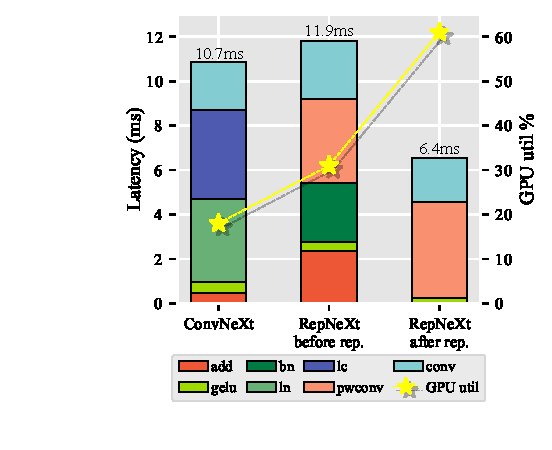
\includegraphics[width=0.7\linewidth]{figs/fig5.pdf}
  \caption{\textbf{Latency decomposition and GPU utilization analysis} of ConvNeXt-T, RepNeXt-u3-T before and after structural re-parameterization. LN and fully connected layers that rely on dimensional transformations take up much latency in ConvNeXt. The former is inherently time-consuming, and the latter is fragmented. Element-wise addition and multi-branching become non-negligible factors affecting the inference speed of RepNeXt in the training time. RepNeXt obtained inference acceleration by tidying up complex structures in the inference time. GPU utilization can reflect the degree of parallelism of a network. The elimination of multi-branch and fragmented structures improves the parallelism of RepNeXt in the inference time, which is another significant factor for its acceleration.}\label{pie}
\end{figure}


\subsection{Ablation study}
\label{sec:ablation}

To compare the impact of each component on performance and efficiency, we modify ConvNeXt into RepNeXt step by step. The accuracy and latency of each intermediate network are recorded, as shown in Table \ref{table:ablation}.

According to Table \ref{table:ablation}, \textbf{1)} A captivating observation is that using fully connected layers is more capable of achieving high performance than using conv layers to implement pointwise conv layers. However, this implementation slows down the inference of the network (but as mentioned earlier, the fully connected layer has the potential to achieve better throughput). The interconversion of fully connected and pointwise conv layers can help you find a better solution. \textbf{2)} The BN layer is still a valuable structure for normalization because it is efficient and can be merged with its adjacent conv layer. The BN layer is only slightly less capable of improving the accuracy of a network than the LN layer because of its local normalization. \textbf{3)} When activation layers are added to the shortcut branch, the accuracy of the network decreases. This is mainly because the number of activations in the network is boosted from $[0, N]$ to $[N,2N]$, where $N$ denotes the number of activations in the original network. This breaks the fewer activations paradigm for high performance ConvNet design. Such an effect may become more evident as $N$ increases. This is a future work that is worth continuing to delve into. \textbf{4)} The comparison between Shortcut-act and RepNeXt reflects the role of RepUnit, which improves the performance with a stronger feature extraction capability. It also confirms that texture bias is also critical to ImageNet classification. \textbf{5)} Structural re-parameterization facilitates stable inference (smaller latency variance) since a cleaner network means less external interference.

\begin{table}[]
\centering
\small
\begin{tabular}{lccc} \hline
Model & Rep. & Latency (ms) & Top-1 acc. \\ \hline
ConvNeXt-T & \ding{56} & 10.7 $\pm$ 2.5 & \textbf{82.1} \\
Lc2pwconv-T & \ding{56} & 10.2 $\pm$ 2.3 & 81.9 \\
Ln2bn-T & \ding{56} & 8.4 $\pm$ 1.9 &  81.8 \\
Shortcut-act-T & \ding{52} & 8.5 $\pm$ 2.1 $\stackrel{r}{\rightarrow}$ 6.4 $\pm$ 1.6 & 81.6 \\
RepNeXt-u3-T & \ding{52} & 11.9 $\pm$ 3.0 $\stackrel{r}{\rightarrow}$ 6.4 $\pm$ 1.6 & \textbf{82.1} \\ \hline
Shortcut-act-S & \ding{52} & 15.3 $\pm$ 2.5 $\stackrel{r}{\rightarrow}$ 11.1 $\pm$ 2.0 & 82.6 \\
RepNeXt-u3-S & \ding{52} & 20.5 $\pm$ 3.7 $\stackrel{r}{\rightarrow}$ 11.1 $\pm$ 2.0 & \textbf{83.1} \\ \hline
Shortcut-act-B & \ding{52} & 16.0 $\pm$ 3.1 $\stackrel{r}{\rightarrow}$ 14.5 $\pm$ 2.2 & 82.9 \\
RepNeXt-u3-B & \ding{52} & 22.4 $\pm$ 3.5 $\stackrel{r}{\rightarrow}$ 14.5 $\pm$ 2.2 & \textbf{83.7} \\ \hline
\end{tabular}
\caption{\textbf{Results of ablation study}. Lc2pwconv is the network using conv layers to implement pointwise conv layers. Ln2bn is the network after replacing LN layers with BN layers. Shortcut-act is the network with activation layers added to shortcut branches. Each of the above operations is done based on the previous one. Only networks that could be shortcut re-parameterized (Rep.) were tested for speed after re-parameterization.}
\label{table:ablation}
\end{table}

\subsection{Efficiency Evaluation}

In application scenarios, commonly used devices are not only GPUs, but also CPUs and end-side devices, so we tested the efficiency of RepNeXt on a variety of different devices, and the results are shown in Table \ref{tab2}. 

The RepNeXt-u3-T in its regular re-parameterized (rRep) and fully re-parameterized (sRep) variants, demonstrates a powerful balance of efficiency and performance. The rRep variant achieves remarkable CPU and GPU efficiency, evidenced by its leading CPU latency of 36.7 milliseconds and GPU throughput of 2052. Meanwhile, the sRep variant, with its advanced GPU optimization, further enhances this efficiency, achieving the lowest GPU latency at 6.4 milliseconds and the lowest Edge latency at 9.3 milliseconds. Moreover, RepNeXts maintain an exceptional level of performance, achieving a Top-1 accuracy rate of 82.1\%, which underscores their capability to deliver high accuracy in addition to their computational efficiency.

Based on the experimental results, it can be concluded that RepNeXt shows excellent or better performance and efficiency on whichever device it is used.

\begin{table*}[h]
\centering
\small
\begin{adjustbox}{center}
\setlength{\tabcolsep}{0.8mm}{
\begin{tabular}{lccccccccc}
\hline
model & Params. & FLOPs & CPU Lat. & CPU Thr. & GPU Lat. & GPU Thr. & Edge Lat. & Edge Thr. & Top-1 acc \% \\ \hline
MobileNetV3-L & 5.4M & 0.4G & \textbf{33.9} & \textbf{486} & 10.8 & \textbf{6052} & 13.35 & \textbf{964} & 75.2 \\
ResNet50 & 26M & 4.1G & 38.1 & 462 & 9.3 & 1548 & 14.99 & \textbf{348} & 77.2 \\
Swin-T & 28M & 4.5G & 101.3 & 97 & 11.2 & 1326 & 20.68 & 199 & 81.3 \\
ConvNeXt-T & 29M & 4.5G & 41.7 & 420 & 10.7 & 1952 & 12.36 & 247 & \textbf{82.1} \\
RepNeXt-u3-T & 29M & 4.5G & 48.2 & 415 & 11.9 & 896 & 17.6 & 173 & \textbf{82.1} \\
RepNeXt-u3-T-rRep & 29M & 4.4G & \textbf{36.7} & \textbf{504} & \textbf{8.5} & \textbf{2052} & \textbf{9.7} & 253 & \textbf{82.1} \\
RepNeXt-u3-T-sRep & 52M & 8.2G & 49.8 & 183 & \textbf{6.4} & 639 & \textbf{9.3} & 168 & \textbf{82.1} \\ \hline
\end{tabular}}
\end{adjustbox}
\caption{Comparison of metrics with models on different hardware devices. The CPU is Intel(R) Xeon(R) Platinum 8260, the GPU device is NVIDIA A100, the edge device is NVIDIA Jetson Orin. Latency (Lat.) is in milliseconds, and throughput (Thr.) is in images/s. Regular and shortcut type re-parameterization are noted as rRep and sRep.}
\label{tab2}
\end{table*}

\section{Limitations}
\label{sec:limitations}

On the one hand, the additional sparse weights introduced by the shortcut re-parameterization sacrifice throughput for faster inference, making RepNeXts more suitable for single-batch inference. On the other hand, the slow convergence of the multi-branch structure makes RepNeXt require more training rounds and longer training time, although sacrificing training time for the sake of inference efficiency is indeed a characteristic of structural re-parametrization. \cite{online} may be possible solutions for improve training efficiency.

\section{Conclusion}
\label{sec:conclusion}

Deploying intelligent recognition models in practical application environment environments faces the challenge of designing models that combine high accuracy with real-time processing efficiency.

We propose RepNeXt. The potential of structural re-parameterization is fully exploited and expanded to obtain superb performance and efficiency. Concretely, we design re-parameterizable RepUnit to efficiently extract multi-scale features, achieving robust performance and enabling more domain adaptations that are difficult to achieve with both Vision Transformers and the large-convolutional-kernel ConvNets, such as low-resolution and fine-grained image recognition tasks. We as well innovatively make a structural re-parameterization of shortcut branches without any constraints, which optimizes the access memory, parallelism, and hardware utilization in the network inference process at the cost of growing a very small number of network parameters (high sparsity parameters), and further improves the real-time inference efficiency of the network.

In fine-grained and low-resolution tasks (ImageWoof and Cifar100), RepNeXt outperforms ResNet50, ConvNeXt-T, and ViT-B by ~3.1\% and ~2.4\%, respectively, in terms of accuracy, and the latency is reduced to 6.4 milliseconds, which emphasizes its adaptability and computational efficiency. In the ImageNet-1K classification task, RepNeXt demonstrates excellent performance that is on par with, if not better than, SOTA models such as Swin Transformer, ConvNeXt and EfficientNet. With the re-parameterized optimization settings, its latency is reduced to 6.4ms and throughput is increased to 2052 images/second, significantly improving computational efficiency. These improvements highlight RepNeXt's ability to deliver high accuracy while maintaining low latency and high throughput. RepNeXt still maintains excellent inference efficiency on devices commonly used in practical application scenarios such as CPUs, GPUs, and end-side devices.

In summary, RepNeXt offers a promising approach to image recognition, blending accuracy with processing efficiency. Through structural re-parameterization, it achieves noteworthy improvements in classification tasks and shows potential for handling specific challenges such as fine-grained and low-resolution image recognition. While RepNeXt demonstrates enhanced performance and inference speed, it also highlights the ongoing need for models that can efficiently balance computational demands with high accuracy. As the field progresses, RepNeXt's contributions are expected to inspire continued research and development, paving the way for future advancements in computer vision and artificial intelligence.

%%===========================================================================================%%
%% If you are submitting to one of the Nature Portfolio journals, using the eJP submission   %%
%% system, please include the references within the manuscript file itself. You may do this  %%
%% by copying the reference list from your .bbl file, paste it into the main manuscript .tex %%
%% file, and delete the associated \verb+\bibliography+ commands.                            %%
%%===========================================================================================%%

\bibliographystyle{plain}
\bibliography{sn-bibliography}% common bib file
%% if required, the content of .bbl file can be included here once bbl is generated
%%\input sn-article.bbl


\end{document}